\documentclass[12pt]{../style-files/ociamthesis}
 
\usepackage{amssymb}
\usepackage{titlesec}
\usepackage{amsmath}
\usepackage{float}
\usepackage{graphicx}
\usepackage{caption}
\usepackage{subfig}
\usepackage{xcolor}
\usepackage[section]{placeins}
\usepackage{mathrsfs}
\usepackage{bm}
\usepackage{stmaryrd}
\usepackage{siunitx}
\usepackage{rotating}
\usepackage[utf8]{inputenc}
\usepackage[round]{natbib}
\usepackage{tikz}
\usetikzlibrary{fadings}
\usetikzlibrary{arrows,shapes, positioning}
\usepackage{booktabs}
\usepackage{multirow}
\usepackage{rotating}
\usepackage{tabularx}
\usepackage{makecell}

%%%%%%%%%%%%%%%%%%%%%%%%%%%%%%%%%%%%%%%%%%%%%%%%%%%%%%%%%%%%%%%%%%%%%%%
% the following is to alter tikz settings to improve springs figure.
\usetikzlibrary{decorations.pathmorphing,calc,patterns}
\makeatletter
\def\pgfdecorationspringstraightlinelength{0.5cm}
\def\pgfdecorationspringnumberofelement{8}
\def\pgfdecorationspringnaturallength{5cm}
\pgfkeys{%
	/pgf/decoration/.cd,
	spring straight line length/.code={%
		\pgfmathsetlengthmacro\pgfdecorationspringstraightlinelength{#1}},
	spring natural length/.code={%
		\pgfmathsetlengthmacro\pgfdecorationspringnaturallength{#1}},
	spring number of element/.store in=\pgfdecorationspringnumberofelement
}

\pgfdeclaredecoration{coil spring}{straight line}{%
	\state{straight line}[%
	persistent precomputation = {%
		% Compute the effective length of the spring (without the length
		% of the two straight lines): \pgfdecorationspringeffectivelength
		\pgfmathsetlengthmacro{\pgfdecorationspringeffectivelength}%
		{\pgfdecoratedpathlength-2*\pgfdecorationspringstraightlinelength}
		% Compute the effective length of one coil pattern:
		% \pgfdecorationspringeffectivelengthofonecoil
		\pgfmathsetlengthmacro{\pgfdecorationspringeffectivelengthofonecoil}%
		{\pgfdecorationspringeffectivelength/\pgfdecorationspringnumberofelement}
	},
	width = \pgfdecorationspringstraightlinelength,
	next state = draw spring]{%
		\pgfpathlineto{%
			\pgfqpoint{%
				\pgfdecorationspringstraightlinelength}{0pt}}
	}
	\state{draw spring}%
	[width=\pgfdecorationspringeffectivelengthofonecoil,
	repeat state=\pgfdecorationspringnumberofelement-1,next state=final]{%
		\pgfpathcurveto
		{\pgfpoint@onspringcoil{0    }{ 0.555}{1}}
		{\pgfpoint@onspringcoil{0.445}{ 1    }{2}}
		{\pgfpoint@onspringcoil{1    }{ 1    }{3}}
		\pgfpathcurveto
		{\pgfpoint@onspringcoil{1.555}{ 1    }{4}}
		{\pgfpoint@onspringcoil{2    }{ 0.555}{5}}
		{\pgfpoint@onspringcoil{2    }{ 0    }{6}}
		\pgfpathcurveto
		{\pgfpoint@onspringcoil{2    }{-0.555}{7}}
		{\pgfpoint@onspringcoil{1.555}{-1    }{8}}
		{\pgfpoint@onspringcoil{1    }{-1    }{9}}
		\pgfpathcurveto
		{\pgfpoint@onspringcoil{0.445}{-1    }{10}}
		{\pgfpoint@onspringcoil{0    }{-0.555}{11}}
		{\pgfpoint@onspringcoil{0    }{ 0    }{12}}
	}
	\state{final}{%
		\pgfpathlineto{\pgfpointdecoratedpathlast}
	}
}

\def\pgfpoint@onspringcoil#1#2#3{%
	\pgf@x=#1\pgfdecorationsegmentamplitude%
	\pgf@x=.5\pgf@x%
	\pgf@y=#2\pgfdecorationsegmentamplitude%
	\pgfmathparse{0.083333333333*\pgfdecorationspringeffectivelengthofonecoil}%
	\pgf@xa=\pgfmathresult pt
	\advance\pgf@x by#3\pgf@xa%
}

\makeatother

\tikzset{%
	Spring/.style = {%
		decoration = {%
			coil spring,
			spring straight line length = 0.2cm,
			% To be added
			spring natural length = #1,
			spring number of element = 4,
			amplitude=2mm},
		decorate,
		very thick},
	Spring/.default = {4cm}}
%
%%%%%%%%%%%%%%%%%%%%%%%%%%%%%%%%%%%%%%%%%%%%%%%%%%%%%%%%%%%%%%%%%%%%%%%%%%%%%%%%

\usepackage{geometry}
 \geometry{
 a4paper,
 left=40mm,
 right=30mm,
 top=30mm,
 bottom=30mm
 }

\definecolor{theblue}{HTML}{0000CD}

% disable this package for printed version
\usepackage[colorlinks=true, linktocpage=true, allcolors=theblue]{hyperref}

\titleformat{\chapter}[display]
  {\bfseries\Large}
  {\filright\MakeUppercase{\chaptertitlename} \Large\thechapter}
  {1ex}
  {}
  [\vspace{1ex} \hrule \vspace{1pt} \hrule]

\newcommand{\adv}{    {\it Adv. Space Res.}} 
\newcommand{\annG}{   {\it Ann. Geophys.}} 
\newcommand{\aap}{    {\it Astron. Astrophys.}}
\newcommand{\aaps}{   {\it Astron. Astrophys. Suppl.}}
\newcommand{\aapr}{   {\it Astron. Astrophys. Rev.}}
\newcommand{\ag}{     {\it Ann. Geophys.}}
\newcommand{\aj}{     {\it Astron. J.}} 
\newcommand{\apj}{    {\it Astrophys. J.}}
\newcommand{\apjl}{   {\it Astrophys. J. Lett.}}
\newcommand{\apss}{   {\it Astrophys. Space Sci.}} 
\newcommand{\cjaa}{   {\it Chin. J. Astron. Astrophys.}} 
\newcommand{\gafd}{   {\it Geophys. Astrophys. Fluid Dyn.}}
\newcommand{\grl}{    {\it Geophys. Res. Lett.}}
\newcommand{\ijga}{   {\it Int. J. Geomagn. Aeron.}}
\newcommand{\jastp}{  {\it J. Atmos. Solar-Terr. Phys.}} 
\newcommand{\jgr}{    {\it J. Geophys. Res.}}
\newcommand{\mnras}{  {\it Mon. Not. Roy. Astron. Soc.}}
\newcommand{\na}{     {\it New Astronomy}}
\newcommand{\nat}{    {\it Nature}}
\newcommand{\pasp}{   {\it Pub. Astron. Soc. Pac.}}
\newcommand{\pasj}{   {\it Pub. Astron. Soc. Japan}}
\newcommand{\pre}{    {\it Phys. Rev. E}}
\newcommand{\solphys}{{\it Solar Phys.}}
\newcommand{\sovast}{ {\it Soviet  Astron.}} 
\newcommand{\ssr}{    {\it Space Sci. Rev.}}
\newcommand{\caa}{    {\it Chinese Astron. Astrohpys.}} 
\newcommand{\apjs}{   {\it Astrophys. J. Suppl.}}
\newcommand{\lrsp}{{\it Living Rev. Solar Phys.}}

\newcommand{\bv}{\mathbf{v}}
\newcommand{\bB}{\mathbf{B}}

\newcommand{\figdirV}{../main/figures/chpt-5/} % where figures are stored


\begin{document}

\baselineskip=18pt

\setcounter{secnumdepth}{3}
\setcounter{tocdepth}{3}

\setcounter{chapter}{4}


% include tex file for chapter
%------------------------------------------------------------------------------
\chapter{Asymmetric waveguides - solar magneto-seismology}
\label{chap: SMS}
%------------------------------------------------------------------------------

%------------------------------------------------------------------------------
\section{Chapter introduction}
\label{sec: SMS intro}
%------------------------------------------------------------------------------


In this chapter, we derive two novel techniques for spatial seismology that use an asymmetric slab waveguide to approximate background parameters. This has applications to solar atmospheric structures that are locally slab-like which have been observed to guide MHD oscillations, such as elongated magnetic bright points \citep{yua_etal14}, prominences \citep{arr_etal12}, and light bridge surges \citep{roy73,shi_etal09} (which have also been named light walls by, \textit{e.g.} \citealp{yan_etal15,yan_etal17,zha_etal17}).

We showed in Chapter~\ref{chap: EVP} that a magnetic slab, with non-magnetic, but asymmetric density and temperatures outside the slab has eigenmodes which can be described as either quasi-sausage or quasi-kink. For quasi-sausage (quasi-kink) modes, the oscillations on each slab interface are in anti-phase (phase). They differ in character from traditional (symmetric) sausage and kink modes by their asymmetry about the centre of the slab due to the amplitude of oscillation on each interface being unequal caused by the asymmetric external environment. This results in quasi-kink modes not necessarily retaining their cross-sectional area and quasi-sausage modes not necessarily having reflection symmetric about the centre line of the slab. The spatial distribution of these waves across the slab, and therefore the extent to which they are modified from the traditional sausage and kink modes, is dependent on the asymmetric background plasma parameters. Consequently, we can use the spatial distribution of these waves to diagnose the waveguide. This is the focus of the present chapter: to derive expressions for proxy parameters that encapsulate this asymmetric spatial distribution and discuss the application to SMS.

Sections~\ref{sec: what is SMS} and~\ref{sec: SMS history} give a definition and brief history of SMS. Sections~\ref{sec: AR} and~\ref{sec: MPS} introduce two new SMS techniques: the Amplitude Ratio Method and the Minimum Perturbation Shift Method. Section~\ref{sec: numerical inversion} discusses in more depth the numerical inversion procedure required to apply these two techniques without having to resort to additional approximations. Section~\ref{sec: SMS discussion} discusses where these techniques can be appropriately applied and Section~\ref{sec: fibrils} records the first use of the Amplitude Ratio Method on solar observations.


\subsection{What is solar magneto-seismology?} \label{sec: what is SMS}

Perpetual bubbling, erupting, and turbulent buffeting of plasma drive ubiquitous magneto-acoustic waves throughout the solar atmosphere. The topology and strength of the magnetic field determines the type and properties of waves present in a given structure. Therefore, by observing these waves and solving an inverse problem, it is possible to make a diagnosis of unknown plasma parameters - a class of techniques known as \textit{solar magneto-seismology} (SMS) \citep{and_etal09,arr12,dem_etal12}. This in turn equips us with more realistic parameters for numerical simulations and give us a better understanding of conditions that lead to, for example, wave energy dissipation, instability, magnetic reconnection, and heating.

SMS techniques can be categorised as either \textit{temporal} or \textit{spatial}. Temporal seismology refers to techniques that estimate a plasma parameter by using the observed frequency, or equivalently the period, of waves. Spatial seismology refers to techniques that estimate a plasma parameter by comparing the observed spatial wave power distribution with the eigenfunctions from a theoretical model. Mathematically, the distinction is that temporal seismology techniques use temporal wave parameters (eigenfrequency) only whereas spatial seismology techniques use spatial or a combination of temporal and spatial wave parameters (eigenfunction).

The flowchart in Figure~\ref{fig: SMS} illustrates the causal chain from identifying wave and equilibrium parameters in observations, combining these with eigenmode analysis from models of the physical system, and using SMS techniques to diagnose previously unknown equilibrium parameters.

\newcommand{\tb}{\textcolor{black}}
\tikzstyle{format} = [draw, rounded corners=.055cm, fill=cyan!20]
\tikzstyle{format2} = [draw, rounded corners=.055cm, fill=red!20]
\begin{figure}
	\begin{tikzpicture}[node distance=1.8cm and 3.3cm, auto, >=latex, align = flush center, ultra thick, on grid=true, font=\small]
	% We need to set at bounding box first. Otherwise the diagram
	% will change position for each frame.
	\path[use as bounding box] (-1.7,-4.1) rectangle (10,2);
	\path node[format] (obs) {
		Observations};
	\path node[below= of obs] (ghost) {};
	\path node[format, below= of ghost] (phys) {
		Physical \\ 
		understanding};
	
	\path node[format2, below right= of obs] (ep) {
		Equilibrium \\ 
		parameters};
	\path (ep) edge[<-] (obs);
	\path node[format, above right= of obs] (wp) {
		Wave \\ 
		parameters}
	edge[<-] (obs);
	
	\path node[format, right= of wp] (tp) {
		Temporal \\ 
		parameters}
	edge[<-] (wp);
	\path node[format, below= of tp] (sp) {
		Spatial \\ 
		parameters}
	edge[<-] (wp)
	edge[<-] (ep);  
	
	\path node[format, right= of phys] (em) {
		Equilibrium \\ 
		models};
	\path (em) edge[<-] (phys);
	
	\path node[format, right= of em] (eig) {
		Eigenmodes}
	edge[<-] (em);
	
	\path node[format, right= of sp] (ts) {
		Temporal \\
		magneto-seismology};
	\path (ts) edge[<-] (tp);
	\node at (6.6,-2) (ghost2) {};
	\draw [->] (ghost2.center) -- (ts);
	\draw (ghost2.center) -- (eig);
	\path node[format, below right= of sp] (ss) {
		Spatial \\
		magneto-seismology};
	\draw [->] (eig) -- (ss);
	\path (ss) edge[<-] (sp);
	
	
	\path (ts) edge[->] (ep);
	\path (ss) edge[->] (ep);
	
	\end{tikzpicture}
	\caption{A flow chart illustrating the causal chain of solar magneto-seismology.}
	\label{fig: SMS}
\end{figure}

Several temporal seismology methods have been employed successfully. \cite{ros70} first suggested that the frequency of oscillations, observed through the fluctuation of synchrotron radiation due to the presence of MHD waves, could be used to diagnose background parameters. Further theoretical development has led to more sophisticated temporal methods including local coronal magnetic field strength estimates using standing kink modes in coronal loops by \cite{nak_etal01}, and using slow sausage and kink modes by \cite{erd_etal08}. The ratio of periods of the fundamental and the first harmonic standing kink mode and its dependence on density stratification has also been well studied \citep{ban_etal07,erd_etal14,yu_etal16}.

Spatial seismology techniques have more recently started demonstrating their efficacy in estimating solar parameters. \cite{uch70} estimated the coronal magnetic structure by comparing Moreton wave observations with the theoretical influence that the coronal magnetic field has on the shape of the Moreton wavefront. More recent eigenfunction methods include utilising the anti-node shift of standing modes in a magnetic flux tube to diagnose its inhomogeneous density stratification \citep{erd_etal07,ver_etal07,erd_etal14}.

In this thesis, we particularly focus on diagnosis of the magnetic field. This is because out of all the solar atmospheric features, the magnetic field is often the most elusive and amongst the most dominant in governing solar atmospheric phenomena. It is insightful to consider SMS techniques are part of a larger umbrella of magnetometry techniques, so that the most appropriate technique can be chosen for a given purpose, and to avoid any implication that the new techniques presented in this thesis are useful in every scenario. This broader class of techniques is outlined in Appendix~\ref{app: magnetometry}.


\subsection{A brief history of solar magneto-seismology} \label{sec: SMS history}

To motivate this chapter's focus on developing new temporal seismology techniques, we list a selection of the major advancements in SMS since its development in Table~\ref{table: SMS history}. There are nine major developments in temporal seismology compared to two major developments in spatial seismology. The dominance of the development of temporal seismology techniques over temporal seismology techniques is striking\footnote{Of course, selection bias could have a role to play here.}. Whilst temporal seismology is growing into a mature field, spatial seismology is in its infancy.

% Define custom callouts to shorten the Author column.
\defcitealias{nak_etal01}{Nakariakov et al.}
\defcitealias{arr_etal11}{Arregui et al.}
\defcitealias{erd_etal08}{Erdelyi et al.}
\begin{table}
	\centering
	\begin{tabularx}{\linewidth}{l l X c}
		\toprule
		Date & Author & Description & Type \\
		\midrule
		1970 & \citeauthor{ros70} & Pulsations in synchrotron radiation caused by MHD waves. & T \\
		1970 & \citeauthor{uch70} & Moreton wavefront morphology used to diagnose coronal magnetic structure. & S \\
		1984 & \citeauthor{rob_etal84} & Introduced the theory of coronal seismology. & T \\
		1995 & \citeauthor{tan95} & Prominence seismology. & T \\
		1999 & \makecell[tl]{\citeauthor{asc_etal99} \\ \citeauthor{nak_etal99}}  & First observations of coronal loop oscillations using TRACE. & N \\
		2001 & \citetalias{nak_etal01} & Period of standing kink mode used to diagnose magnetic field strength in coronal loops. & T \\
		2002 & \citeauthor{goo_etal02} & Damping time scales (assuming exponential damping profile) used to estimate density variation across a coronal loop. & T \\
		2005 & \citeauthor{and_etal05} & Density stratification deduced from the period ratio of the first two standing kink harmonics. & T \\
		2007 & \citeauthor{ver_etal07} & Anti-node shift used to diagnose density stratification along the loop. & S \\
		2008 & \citetalias{erd_etal08} & Seismology of slow standing modes in coronal loops. & T \\
		2011 & \citetalias{arr_etal11} & Probabilistic coronal seismology inversion using Bayesian statistics. & N \\
		2013 & \citeauthor{pas_etal13} & A combination of Gaussian and exponential damping of kink modes used to estimate loop density. & T \\
		2017 & \citeauthor{lon_etal17} & Dynamic coronal seismology, \textit{i.e.} diagnosing the magnetic field strength changing in time and across a large portion of the solar atmosphere. Using the methodology developed by \cite{mor_etal15}. & T \\
		\bottomrule
	\end{tabularx}
	\caption{History of solar magneto-seismology development. The \textit{type} column refers to whether the development is in temporal seismology (T), spatial seismology (S), or neither (N).}
	\label{table: SMS history}
\end{table}

Why has spatial seismology lagged behind? There are several plausible answers to this questions. Both ground-based and space-bourne solar telescopes suffer from limitations in spatial resolution. The most significant increases in spatial resolution come from increasing telescope's aperture size. Space-bourne telescopes are limited in this regard because larger aperture size means a larger spacecraft is required to deliver the telescope into orbit. This comes at significant extra cost. Ground-based telescopes suffer from limitations on their spatial resolution from seeing effects, although this has been partially overcome in the era of adaptive optics. These limitations have allowed faster improvements in temporal resolution compared to spatial resolution, therefore the measurement errors in temporal parameters tend to be lower than those in spatial parameters. This means that temporal seismology inversions tend to have lower errors that propagate through from input errors than spatial seismology inversions.

A second plausible explanation is that the development of spatial seismology techniques tends to require more sophisticated MHD wave modelling than temporal seismology techniques. In general, spatial seismology techniques exploit some observational consequence of a deviation of a waveguide from its most simple counterpart to estimate an unknown parameter. For example, the anti-node shift method uses the shift in position (observational consequence of density non-uniformity) of the anti-nodes of standing modes of coronal loops, due to enhanced density in the loop foot-points (deviation from simple model of a uniform flux tube) to estimate the foot-point density (unknown parameter). An interpretation the techniques we will develop in Sections~\ref{sec: AR} and~\ref{sec: MPS} using this framing is that these techniques use the amplitude ratio or minimum perturbation shift (observational consequences of waveguide asymmetry) which exist due to the asymmetry of the waveguide (deviation from the simple symmetric slab model) which are proxies for the strength of the magnetic field (unknown parameter).


%------------------------------------------------------------------------------
\section{Amplitude Ratio}
\label{sec: AR}
%------------------------------------------------------------------------------

The aim of this section is to derive an expression for the ratio of the oscillation amplitude on each interface of an asymmetric magnetic slab in terms of the wave parameters and plasma parameters of the system, then demonstrate how this parameter can be utilised to diagnose background parameters. We focus on estimating the Alfv\'{e}n speed since it is the the most difficult of all our background parameters to measure using traditional methods. We do this by first deriving expressions for the eigenfunctions\footnote{That is, the distribution of the oscillation amplitude across the waveguide.} of quasi-sausage and quasi-kink modes, using them to derive expressions for the Amplitude Ratio, and then by making suitable approximations, we can solve the inverse problem for the Alfv\'{e}n speed. Numerical inversion procedures for the Amplitude Ratio Method are discussed in Section~\ref{sec: numerical inversion}.

\subsection{Deriving an expression for the Amplitude Ratio} \label{sec: AR derivation}

Consider an asymmetric magnetic slab in a non-magnetic environment, as studied in Section~\ref{sec: EVP non-mag} and by \cite{all_etal17}. In this section, we denote the Alfv\'{e}n speed inside the slab as $v_\textrm{A}$ rather than $v_{A0}$ for brevity because it is the only Alfv\'{e}n speed in the system since we have let the external plasma be non-magnetic.

In Section~\ref{sec: EVP non-mag}, it was shown that trapped magneto-acoustic modes propagating along an asymmetric magnetic slab have velocity perturbation in the $x$-direction given by $v_x(x,y,z,t) = \widehat{v}_x(x)e^{i(kz-\omega t)}$, where $\omega$ and $k$ are the angular frequency and wavenumber, and
\begin{equation}
\hat{v}_x(x)=
\begin{cases}
A(\cosh{m_1x} + \sinh{m_1x}) & \text{if } x < -x_0, \\
B\cosh{m_0x} + C\sinh{m_0x} & \text{if } |x| \leq x_0, \\
D(\cosh{m_2x} - \sinh{m_2x}) & \text{if } x > x_0, \label{vsoln}
\end{cases}
\end{equation}
where
\begin{equation}
m_0^2 = \frac{(k^2v_\textrm{A}^2 - \omega^2)(k^2c_0^2 - \omega^2)}{(c_0^2 + v_\textrm{A}^2)(k^2c_{T0}^2-\omega^2)}, \qquad c_{T0}^2 = \frac{c_0^2v_\textrm{A}^2}{c_0^2 + v_\textrm{A}^2}, \label{m0}
\end{equation}
\begin{equation}
m_j^2 = k^2 - \frac{\omega^2}{c_j^2}, \quad \text{for $j = 1, 2$,} \label{m1,2}
\end{equation}
and $A, B, C$, and $D$ are arbitrary constants (with respect to $x$). Therefore, to derive expressions for the eigenfunctions, we need to determine these constants. They can be determined, to within one degree of freedom, using the boundary conditions of continuity in total pressure and transversal velocity component across the slab boundaries at $x = \pm x_0$. Applying these four boundary conditions retrieves four coupled linear homogeneous algebraic equations in the four unknowns, namely
\begin{equation}
\left(
\begin{matrix}
c_1 - s_1 &-c_0                       &s_0                        &0 \\
0       &c_0                        &s_0                        &s_2 - c_2 \\
\Lambda_1(c_1 - s_1)       &\Lambda_0s_0 &-\Lambda_0c_0  &0 \\
0       &\Lambda_0s_0                          &\Lambda                   _0c_0 &-\Lambda_2(s_2 - c_2)
\end{matrix}
\right)
\left(
\begin{matrix}
A \\
B \\
C \\
D
\end{matrix}
\right)
=
\left(
\begin{matrix}
0 \\
0 \\
0 \\
0
\end{matrix}
\right),
\label{coefmatrix}
\end{equation}
where
\begin{equation}
\Lambda_0 = -\frac{i\rho_0(k^2v_\textrm{A}^2 - \omega^2)}{m_0\omega}, \quad \Lambda_1 = \frac{i\rho_1\omega}{m_1}, \quad \text{and} \quad \Lambda_2 = \frac{i\rho_2\omega}{m_2}, \label{Lambdas}
\end{equation}
and $c_i = \cosh{m_ix_0}$ and $s_i = \sinh{m_ix_i}$, for $i = 0, 1, 2$. Ensuring that this matrix has a vanishing determinant gives us the dispersion relation,
\begin{equation}
(\Lambda_0c_0 + \Lambda_2s_0)(\Lambda_0s_0 + \Lambda_1c_0) + (\Lambda_0c_0 + \Lambda_1s_0)(\Lambda_0s_0 + \Lambda_2c_0) = 0. \label{disp rel}
\end{equation}
By satisfying this relation, we gain one degree of freedom in the system of Equations~\eqref{coefmatrix}, which leaves one of the constants $B$ or $C$ arbitrary. This leads to two types of solution: \textit{quasi-sausage} and \textit{quasi-kink} modes.

Firstly, for quasi-sausage modes, by letting $C$ be arbitrary the other constants $A$, $B$, and $D$ can be determined as
\begin{align}
A =& \frac{1}{c_1 - s_1}(Bc_0 - Cs_0), \label{constA C} \\ 
D =& \frac{1}{c_2 - s_2}(Bc_0 + Cs_0), \label{constD C}
\end{align}
where
\begin{equation}
B = \frac{\Lambda_0c_0 + \Lambda_1s_0}{\Lambda_0s_0 + \Lambda_1c_0}C = -\frac{\Lambda_0c_0 + \Lambda_2s_0}{\Lambda_0s_0 + \Lambda_2c_0}C. \label{constB C}
\end{equation}
The second formulation of $B$ in Equation~\eqref{constB C} is found by utilising the dispersion relation, Equation~\eqref{disp rel}. A substitution of these values, using the first form of $B$ in Equation~\eqref{constB C}, into the velocity solution, Equation~\eqref{vsoln}, evaluated at the slab boundaries, yields
\begin{align}
\hat{v}_x(x_0) =& Bc_0 + Cs_0 = \frac{2\Lambda_1 + \Lambda_0\left(\tau_0 + \frac{1}{\tau_0}\right)}{\Lambda_0 + \Lambda_1\frac{1}{\tau_0}}Cc_0, \label{vx_01 C} \\
\hat{v}_x(-x_0) =& Bc_0 - Cs_0 = \frac{\Lambda_0}{\Lambda_0 + \Lambda_1\frac{1}{\tau_0}}C/s_0, \label{v-x_01 C}
\end{align}
where $\tau_0 = \tanh{m_0x_0}$. Similarly, using the second form of $B$ in Equation~\eqref{constB C} yields
\begin{align}
\hat{v}_x(x_0) =& \frac{-\Lambda_0}{\Lambda_0 + \Lambda_2\frac{1}{\tau_0}}C/s_0, \label{vx_02 C} \\
\hat{v}_x(-x_0) =& \frac{-2\Lambda_2 - \Lambda_0\left(\tau_0 + \frac{1}{\tau_0}\right)}{\Lambda_0 + \Lambda_2\frac{1}{\tau_0}}Cc_0. \label{v-x_02 C}
\end{align}
These forms are equivalent. Notice that the horizontal velocity perturbation amplitude, $\hat{v}_x$, is, more precisely, the \emph{signed} amplitude, where a positive (negative) value indicates perturbation in the positive (negative) $x$-direction. This will be important for the inversion procedure.

Secondly, for quasi-kink modes, by letting $B$ be arbitrary, the other constants $A$, $C$, and $D$ can be determined in terms of $B$ as
\begin{align}
A =& \frac{1}{c_1 - s_1}(Bc_0 - Cs_0), \label{constA B} \\ 
D =& \frac{1}{c_2 - s_2}(Bc_0 + Cs_0), \label{constD B}
\end{align}
where
\begin{equation}
C = \frac{\Lambda_0s_0 + \Lambda_1c_0}{\Lambda_0c_0 + \Lambda_1s_0}B = -\frac{\Lambda_0s_0 + \Lambda_2c_0}{\Lambda_0c_0 + \Lambda_2s_0}B. \label{constB B}
\end{equation}
A substitution of these values, using the first form of $C$ in Equation~\eqref{constB B}, into Equation~\eqref{vsoln}, evaluated at the slab boundaries, yields
\begin{align}
\hat{v}_x(x_0) =& \frac{2\Lambda_1 + \Lambda_0\left(\tau_0 + \frac{1}{\tau_0}\right)}{\Lambda_0 + \Lambda_1\tau_0}Bs_0, \label{vx_01 B} \\
\hat{v}_x(-x_0) =& \frac{\Lambda_0}{\Lambda_0 + \Lambda_1\tau_0}B/c_0. \label{v-x_01 B}
\end{align}
Using the second form of $C$ in Equation~\eqref{constB B} yields
\begin{align}
\hat{v}_x(x_0) =& \frac{\Lambda_0}{\Lambda_0 + \Lambda_2\tau_0}B/c_0, \label{vx_02 B} \\
\hat{v}_x(-x_0) =& \frac{2\Lambda_2 + \Lambda_0\left(\tau_0 + \frac{1}{\tau_0}\right)}{\Lambda_0 + \Lambda_2\tau_0}Bs_0. \label{v-x_02 B}
\end{align}

\begin{figure}
	\makebox[\textwidth][c]{
		\subfloat[]{
				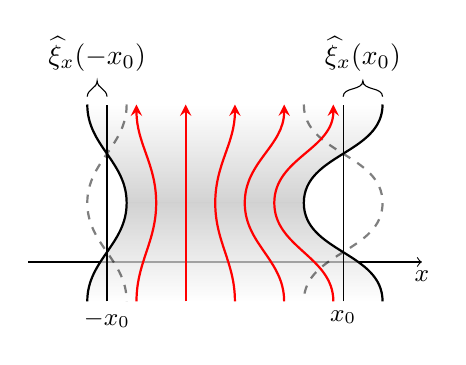
\begin{tikzpicture}
				\draw [->] (1,0) -- (6,0);
				
				\shade[bottom color=lightgray,top color=white, opacity=0.7] (1.75,2) to [out=-90,in=90] (2.25,0.75) to (4.5,0.75) to [out=90,in=-90] (5.5,2) to (1.75,2);
				
				\shade[bottom color=white,top color=lightgray, opacity=0.7] (2.25,0.75) to (4.5,0.75) to [out=-90,in=90] (5.5,-0.5) to (1.75,-0.5) to [out=90,in=-90] (2.25,0.75);
				
				\draw [thick] (1.75,2) to [out=-90,in=90] (2.25,0.75) to [out=-90,in=90] (1.75,-0.5);
				\draw [thick, dashed, opacity=0.5] (4.5,2) to [out=-90,in=90] (5.5,0.75) to [out=-90,in=90] (4.5,-0.5);
				
				\draw [thick, red, -stealth] (2.375,-0.5) to [out=90,in=-90] (2.625, 0.75) to [out=90,in=-90] (2.375,2);
				\draw [thick, red, -stealth] (3,-0.5) to [out=90,in=-90] (3, 0.75) to [out=90,in=-90] (3,2);
				\draw [thick, red, -stealth] (3.625,-0.5) to [out=90,in=-90] (3.375, 0.75) to [out=90,in=-90] (3.625,2);
				\draw [thick, red, -stealth] (4.25,-0.5) to [out=90,in=-90] (3.75, 0.75) to [out=90,in=-90] (4.25,2);
				\draw [thick, red, -stealth] (4.875,-0.5) to [out=90,in=-90] (4.125, 0.75) to [out=90,in=-90] (4.875,2);
				
				\draw [thick, dashed, opacity=0.5] (2.25,2) to [out=-90,in=90] (1.75,0.75) to [out=-90,in=90] (2.25,-0.5);
				\draw [thick] (5.5,2) to [out=-90,in=90] (4.5,0.75) to [out=-90,in=90] (5.5,-0.5);
				
				% % % % % % % % % % % % % % % % % % % % % % % % % %
				
				%\draw [->] (0,0) -- (0,2);
				
				%\node at (1,1) {$\rho_1$};
				%\node at (6,1) {$\rho_2$};
				%\node [right] at (2.95,1.3) {$\rho_0$};
				
				\draw [-] (1.75, 2.1) to [out=90, in=-90] (1.875, 2.3) to [out=-90, in=90] (2, 2.1);
				\draw [-] (5, 2.1) to [out=90, in=-90] (5.25, 2.3) to [out=-90, in=90] (5.5, 2.1);
				
				\node [above] at (1.875,2.3) {$\widehat{\xi}_x(-x_0)$};
				\node [above] at (5.25, 2.3) {$\widehat{\xi}_x(x_0)$};
				
				\small
				\node [below] at (2,-0.5) {$-x_0$};
				\node [below] at (5,-0.5) {$x_0$};
				
				%\node [left] at (0,2) {$z$};
				\node [below] at (6,0) {$x$};
				\draw [-] (2,-0.5) -- (2,2);
				\draw [-] (5,-0.5) -- (5,2);
				\end{tikzpicture} 
			\label{fig: RA saus}}
		
		
		\subfloat[]{
				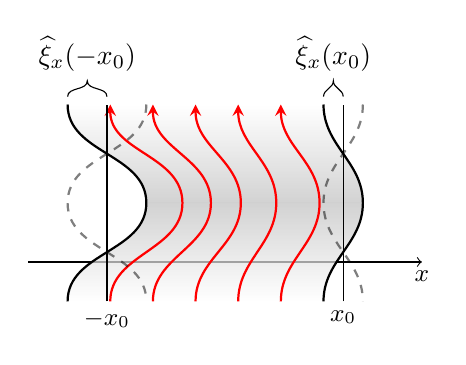
\begin{tikzpicture}
				\draw [->] (1,0) -- (6,0);
				
				\shade[bottom color=lightgray,top color=white, opacity=0.7] (1.5,2) to [out=-90,in=90] (2.5,0.75) to (5.25,0.75) to [out=90,in=-90] (4.75,2) to (1.5,2);
				
				\shade[bottom color=white,top color=lightgray, opacity=0.7] (2.5,0.75) to (5.25,0.75) to [out=-90,in=90] (4.75,-0.5) to (1.5,-0.5) to [out=90,in=-90] (2.5,0.75);
				
				\draw [thick] (1.5,2) to [out=-90,in=90] (2.5,0.75) to [out=-90,in=90] (1.5,-0.5);
				\draw [thick] (4.75,2) to [out=-90,in=90] (5.25,0.75) to [out=-90,in=90] (4.75,-0.5);
				
				%\draw [thick, red, -stealth] (2.0417,-0.5) to [out=90,in=-90] (2.9583, 0.75) to [out=90,in=-90] (2.0417,2);
				%\draw [thick, red, -stealth] (2.5833,-0.5) to [out=90,in=-90] (3.4167, 0.75) to [out=90,in=-90] (2.5833,2);
				%\draw [thick, red, -stealth] (3.125,-0.5) to [out=90,in=-90] (3.875, 0.75) to [out=90,in=-90] (3.125,2);
				%\draw [thick, red, -stealth] (3.6667,-0.5) to [out=90,in=-90] (4.3333, 0.75) to [out=90,in=-90] (3.6667,2);
				%\draw [thick, red, -stealth] (4.2083,-0.5) to [out=90,in=-90] (4.7917, 0.75) to [out=90,in=-90] (4.2083,2);
				
				\draw [thick, red, -stealth] (2.0417,-0.5) to [out=90,in=-90] (2.9583, 0.75) to [out=90,in=-90] (2.0417,2);
				\draw [thick, red, -stealth] (2.5833,-0.5) to [out=90,in=-90] (3.32, 0.75) to [out=90,in=-90] (2.5833,2);
				\draw [thick, red, -stealth] (3.125,-0.5) to [out=90,in=-90] (3.7, 0.75) to [out=90,in=-90] (3.125,2);
				\draw [thick, red, -stealth] (3.6667,-0.5) to [out=90,in=-90] (4.15, 0.75) to [out=90,in=-90] (3.6667,2);
				\draw [thick, red, -stealth] (4.2083,-0.5) to [out=90,in=-90] (4.7, 0.75) to [out=90,in=-90] (4.2083,2);
				
				\draw [thick, dashed, opacity=0.5] (2.5,2) to [out=-90,in=90] (1.5,0.75) to [out=-90,in=90] (2.5,-0.5);
				\draw [thick, dashed, opacity=0.5] (5.25,2) to [out=-90,in=90] (4.75,0.75) to [out=-90,in=90] (5.25,-0.5);
				
				% % % % % % % % % % % % % % % % % % % % % % % % % %
				
				\draw [-] (1.5, 2.1) to [out=90, in=-90] (1.75, 2.3) to [out=-90, in=90] (2., 2.1);
				\draw [-] (4.75, 2.1) to [out=90, in=-90] (4.875, 2.3) to [out=-90, in=90] (5., 2.1);
				
				\node [above] at (1.75,2.3) {$\widehat{\xi}_x(-x_0)$};
				\node [above] at (4.875, 2.3) {$\widehat{\xi}_x(x_0)$};
				
				\small
				\node [below] at (2,-0.5) {$-x_0$};
				\node [below] at (5,-0.5) {$x_0$};
				
				%\node [left] at (0,2) {$z$};
				\node [below] at (6,0) {$x$};
				\draw [-] (2,-0.5) -- (2,2);
				\draw [-] (5,-0.5) -- (5,2);
				\end{tikzpicture} 
			\label{fig: RA kink}}}
	\caption{Illustration of the difference in amplitude of oscillation on each boundary of the slab for~\protect\subref{fig: RA saus}~quasi-sausage and~\protect\subref{fig: RA kink}~quasi-kink modes.}
	\label{fig: RA}
\end{figure}

We now define the \emph{amplitude ratio}, $R_\textrm{A} := \hat{\xi}_x(x_0) / \hat{\xi}_x(-x_0)$, as the ratio of the amplitude of oscillation of the left interface ($x = x_0$) to that of the right interface ($x = -x_0$) (see Figure~\ref{fig: RA}). Given that ${\hat{\xi}_x(x) = i\hat{v}_x(x) / \omega}$, we also have $R_\textrm{A} = \hat{v}_x(x_0) / \hat{v}_x(-x_0)$. Firstly, using Equations~\eqref{v-x_01 C} and~\eqref{vx_02 C}, the amplitude ratio for quasi-sausage modes is
\begin{align}
R_A &= -\frac{\Lambda_0 + \Lambda_1\frac{1}{\tau_0}}{\Lambda_0 + \Lambda_2\frac{1}{\tau_0}} \notag \\
&= -\frac{\rho_1m_2}{\rho_2m_1}\left[\frac{(k^2v_\textrm{A}^2 - \omega^2)m_1\frac{\rho_0}{\rho_1} - \omega^2m_0\coth{m_0x_0}}{(k^2v_\textrm{A}^2 - \omega^2)m_2\frac{\rho_0}{\rho_2} - \omega^2m_0\coth{m_0x_0}}\right]. \label{AR saus}
\end{align}
Using Equations~\eqref{v-x_01 B} and~\eqref{vx_02 B}, the corresponding expression for quasi-kink modes can be obtained, namely
\begin{align}
R_\textrm{A} &= \frac{\Lambda_0 + \Lambda_1\tau_0}{\Lambda_0 + \Lambda_2\tau_0} \notag \\
&= \frac{\rho_1m_2}{\rho_2m_1}\left[\frac{(k^2v_\textrm{A}^2 - \omega^2)m_1\frac{\rho_0}{\rho_1} - \omega^2m_0\tanh{m_0x_0}}{(k^2v_\textrm{A}^2 - \omega^2)m_2\frac{\rho_0}{\rho_2} - \omega^2m_0\tanh{m_0x_0}}\right]. \label{AR kink}
\end{align}
As expected, Equations~\eqref{AR saus} and~\eqref{AR kink} reduce to $R_\textrm{A} = -1$ and $R_\textrm{A} = 1$ for sausage and kink modes, respectively, when the slab is symmetric.

To obtain an approximation for the Alfv\'{e}n speed analytically, an approximation such as these must be applied. The following subsections give the analytical inversion for the Alfv\'{e}n speed, $v_\textrm{A}$, of equations~\eqref{AR saus} and~\eqref{AR kink} under the thin slab, wide slab, incompressible plasma, and low-beta approximations. A numerical inversion procedure that requires no further approximation is discussed in Section~\ref{sec: numerical inversion}. Note that we restrict the parameter inversions to surface modes only, thereby omitting body modes, because the eigenfrequencies and eigenfunctions of body modes are not significantly effected by asymmetry in the external plasma (see Section~\ref{sec: EVP non-mag}) so they are not useful for parameter inversion.


\subsection{Thin slab approximation} \label{sec: AR thin slab}
For surface modes in the thin slab approximation, $kx_0 \ll 1$, \cite{rob81b} showed that $m_0x_0 \ll 1$. Therefore, to quadratic order, $\tanh{m_0x_0} \approx m_0x_0$, and the amplitude ratio for a quasi-sausage surface mode in a thin slab reduces to
\begin{equation}
R_\textrm{A} = -\frac{\rho_1m_2}{\rho_2m_1}\left[\frac{(k^2v_\textrm{A}^2 - \omega^2)m_1x_0\frac{\rho_0}{\rho_1} - \omega^2}{(k^2v_\textrm{A}^2 - \omega^2)m_2x_0\frac{\rho_0}{\rho_2} - \omega^2}\right], 
\end{equation}
which can be rearranged to give the analytical expression
\begin{equation}
v_\textrm{A}^2 = \frac{\omega^2}{k^2} \left[1 + \frac{1}{x_0} \left(\frac{R_\textrm{A}\frac{\rho_2}{\rho_0m_2} + \frac{\rho_1}{\rho_0m_1}}{R_\textrm{A} + 1}\right)\right].
\end{equation}
The amplitude ratio for a thin slab quasi-kink surface mode reduces to
\begin{equation}
R_\textrm{A} = \frac{\rho_1m_2}{\rho_2m_1} \left[\frac{(k^2v_\textrm{A}^2 - \omega^2)m_1\frac{\rho_0}{\rho_1} - \omega^2m_0^2x_0}{(k^2v_\textrm{A}^2 - \omega^2)m_2\frac{\rho_0}{\rho_2} - \omega^2m_0^2x_0}\right], 
\end{equation}
which can be rearranged to give the analytical expression
\begin{equation}
v_\textrm{A}^2 = \frac{\omega^2}{k^2} \left[\frac{c_0^2}{c_0^2 - \frac{\omega^2}{k^2}} + k^2x_0\left(\frac{R_\textrm{A}\frac{\rho_2}{\rho_0m_2} - \frac{\rho_1}{\rho_0m_1}}{R_\textrm{A} - 1}\right)\right]. \label{AR soln kink thin}
\end{equation}

In a thin asymmetric slab, the fast quasi-kink surface mode degenerates due to a cut-off by the external sound speeds becoming distinct \citep{all_etal17} and the slow quasi-kink surface mode has a phase speed that approaches zero in the thin slab limit (see Section~\ref{sec: thin slab}). Therefore, to a good approximation the phase speed is much less than the internal sound speed ($\omega/k \ll c_0$) therefore Equation~\eqref{AR soln kink thin} simplifies to
\begin{equation}
v_\textrm{A}^2 = \frac{\omega^2}{k^2} \left[1 + k^2x_0\left(\frac{R_\textrm{A}\frac{\rho_2}{\rho_0m_2} - \frac{\rho_1}{\rho_0m_1}}{R_\textrm{A} - 1}\right)\right]. \label{AR soln kink thin simplified}
\end{equation}

\subsection{Wide slab approximation} \label{sec: AR wide slab}
The wide slab approximation applies when the slab width is much larger than the wavelength, that is when $kx_0 \gg 1$. In Section~\ref{sec: wide slab}, we showed that the surface mode solutions of a wide asymmetric slab are just the surface modes that propagate along each interface independently.

This is analogous to the mechanical example introduced in Section~\ref{sec: mechanical example}. When the two masses are decoupled by removing the middle spring, equivalently setting $k_0 = 0$, each mass oscillates independently at the natural frequency of that side of the spring-mass system (Figure~\ref{fig: wide slab mechanical analogy}). This decoupling provides a good analogy to the wide slab limit for the magnetic slab. In a wide slab, each interface is effectively \textit{decoupled} and oscillates at its own natural frequency, independent of the other interface. Given that we are considering magneto-acoustic waves, there are two restoring forces, the magnetic tension force and the pressure gradient force, which means that each independent interface has two natural frequencies, corresponding to the fast and slow magneto-acoustic modes. With this understanding of the modes in the wide slab limit, the amplitude ratio, $R_\textrm{A}$, is either $0$ or $\pm\infty$, depending on which interface the wave is propagating and is therefore not useful for magneto-seismology.

\begin{figure}
	\makebox[\textwidth][c]{
		\subfloat[Coupled equilibrium]{\scalebox{0.9}{
				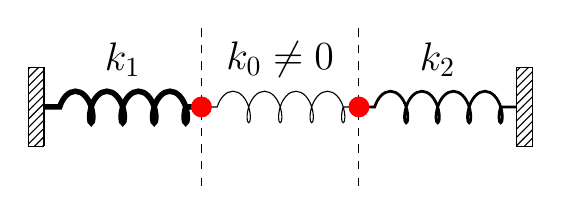
\begin{tikzpicture}
				\filldraw[pattern=north east lines] (0,-0.5) -| (-0.2,0.5) -| (0,-0.5);
				\filldraw[pattern=north east lines] (6,-0.5) -| (6.2,0.5) -| (6,-0.5);
				\draw[Spring, line width=2] (0,0) -- (2,0);
				\draw[Spring, thin] (2,0) -- (4,0);
				\draw[Spring, line width=1] (4,0) -- (6,0);
				
				\draw [dashed] (2,1) -- (2,-1);
				\draw [dashed] (4,1) -- (4,-1);
				
				\draw (2,0) node [fill=red,circle,scale=0.8] {};
				\draw (4,0) node [fill=red,circle,scale=0.8] {};
				
				\Large
				\draw (1,0.6) node [] {$k_1$};
				\draw (3,0.6) node [] {$k_0 \neq 0$};
				\draw (5,0.6) node [] {$k_2$};
				\end{tikzpicture}
		}}
		
		\subfloat[Uncoupled equilibrium]{\scalebox{0.9}{
				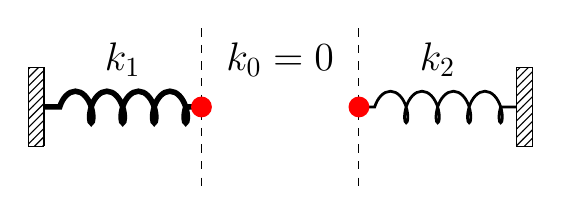
\begin{tikzpicture}
				\filldraw[pattern=north east lines] (0,-0.5) -| (-0.2,0.5) -| (0,-0.5);
				\filldraw[pattern=north east lines] (6,-0.5) -| (6.2,0.5) -| (6,-0.5);
				\draw[Spring, line width=2] (0,0) -- (2,0);
				%\draw[Spring, thin] (2,0) -- (4,0);
				\draw[Spring, line width=1] (4,0) -- (6,0);
				
				\draw [dashed] (2,1) -- (2,-1);
				\draw [dashed] (4,1) -- (4,-1);
				
				\draw (2,0) node [fill=red,circle,scale=0.8] {};
				\draw (4,0) node [fill=red,circle,scale=0.8] {};
				
				\Large
				\draw (1,0.6) node [] {$k_1$};
				\draw (3,0.6) node [] {$k_0 = 0$};
				\draw (5,0.6) node [] {$k_2$};
				\end{tikzpicture}
	}}}
	
	\makebox[\textwidth][c]{
		\subfloat[Uncoupled left oscillation]{\scalebox{0.9}{
				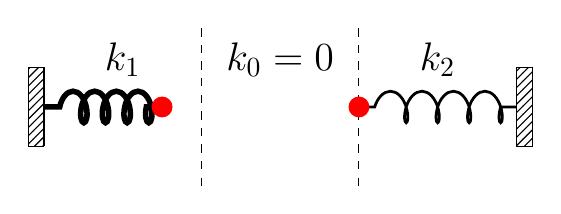
\begin{tikzpicture}
				\filldraw[pattern=north east lines] (0,-0.5) -| (-0.2,0.5) -| (0,-0.5);
				\filldraw[pattern=north east lines] (6,-0.5) -| (6.2,0.5) -| (6,-0.5);
				\draw[Spring, line width=2] (0,0) -- (1.5,0);
				%\draw[Spring, thin] (2,0) -- (4,0);
				\draw[Spring, line width=1] (4,0) -- (6,0);
				
				\draw [dashed] (2,1) -- (2,-1);
				\draw [dashed] (4,1) -- (4,-1);
				
				\draw (1.5,0) node [fill=red,circle,scale=0.8] {};
				\draw (4,0) node [fill=red,circle,scale=0.8] {};
				
				\Large
				\draw (1,0.6) node [] {$k_1$};
				\draw (3,0.6) node [] {$k_0 = 0$};
				\draw (5,0.6) node [] {$k_2$};
				\end{tikzpicture}
		}}
		
		\subfloat[Uncoupled right oscillation]{\scalebox{0.9}{
				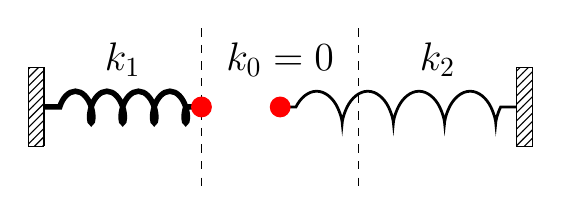
\begin{tikzpicture}
				\filldraw[pattern=north east lines] (0,-0.5) -| (-0.2,0.5) -| (0,-0.5);
				\filldraw[pattern=north east lines] (6,-0.5) -| (6.2,0.5) -| (6,-0.5);
				\draw[Spring, line width=2] (0,0) -- (2,0);
				%\draw[Spring, thin] (2,0) -- (4,0);
				\draw[Spring, line width=1] (3,0) -- (6,0);
				
				\draw [dashed] (2,1) -- (2,-1);
				\draw [dashed] (4,1) -- (4,-1);
				
				\draw (2,0) node [fill=red,circle,scale=0.8] {};
				\draw (3,0) node [fill=red,circle,scale=0.8] {};
				
				\Large
				\draw (1,0.6) node [] {$k_1$};
				\draw (3,0.6) node [] {$k_0 = 0$};
				\draw (5,0.6) node [] {$k_2$};
				\end{tikzpicture}
	}}}
	\caption{Mechanical example showing weak and zero coupling between the masses. This provides an analogy to the wide slab approximation of an asymmetric magnetic slab, in which case the interfaces on each side of the slab oscillate independently.}
	\label{fig: wide slab mechanical analogy}
\end{figure}


\subsection{Incompressible Approximation} \label{sec: AR incomp}

If the plasma is incompressible, the sound speeds become unbounded, so that $m_j \approx k$ for $j = 0, 1, 2$. Under this approximation, the amplitude ratios for quasi-sausage modes (top) and quasi-kink modes (bottom) reduce to
\begin{align}
R_\textrm{A} &= \left(\substack{- \\ +}\right) \frac{\rho_1}{\rho_2} \left[ \frac{(k^2v_\textrm{A}^2 - \omega^2)k\frac{\rho_0}{\rho_1} - \omega^2k \left(\begin{matrix} \coth \\ \tanh \end{matrix}\right)(kx_0)}{(k^2v_\textrm{A}^2-\omega^2)k\frac{\rho_0}{\rho_2}-\omega^2k \left(\begin{matrix} \coth \\ \tanh \end{matrix}\right)(kx_0)} \right].
\end{align}
These equations have solutions for $v_\textrm{A}$ given by
\begin{equation}
v_\textrm{A}^2 = \frac{\omega^2}{k^2} \left[ 1 + \left( \frac{R_\textrm{A} \frac{\rho_2}{\rho_0} \left(\substack{+ \\ -}\right) \frac{\rho_1}{\rho_0}}{R_\textrm{A} \left(\substack{+ \\ -}\right) 1} \right) \left(\begin{matrix} \coth \\ \tanh \end{matrix}\right) (kx_0)\right].
\end{equation}


\subsection{Low-Beta Approximation} \label{sec: AR low-beta}

For a low-beta plasma ($\beta = 2\mu_0p_0/B_0^2 \ll 1$), the magnetic pressure dominates the kinetic plasma pressure and the Alfv\'{e}n speed, $v_\textrm{A}$, dominates the sound speed, $c_0$. Therefore, $m_0^2 \approx k^2 - \omega^2/v_\textrm{A}^2$. For waves with phase speed much less than the Alfv\'{e}n speed, a further approximation of $m_0^2 \approx k^2$ can be made, in which case, the amplitude ratios for quasi-sausage modes (top) and quasi-kink modes (bottom) reduce to
\begin{align}
R_\textrm{A} &= \left(\substack{- \\ +}\right) \frac{\rho_1m_2}{\rho_2m_1} \left[ \frac{(k^2v_\textrm{A}^2 - \omega^2)m_1\frac{\rho_0}{\rho_1} - \omega^2k \left(\begin{matrix} \coth \\ \tanh \end{matrix}\right)(kx_0)}{(k^2v_\textrm{A}^2 - \omega^2)m_2\frac{\rho_0}{\rho_2} - \omega^2k \left(\begin{matrix} \coth \\ \tanh \end{matrix}\right)(kx_0)} \right].
\end{align}
These equations can be solved for $v_\textrm{A}$ to give
\begin{equation}
v_\textrm{A}^2 = \frac{\omega^2}{k^2} \left[1 + k \left( \frac{ \frac{\rho_1}{\rho_0m_1} \left(\substack{+ \\ -}\right) R_\textrm{A}\frac{\rho_2}{\rho_0m_2}}{1 \left(\substack{+ \\ -}\right) R_\textrm{A}} \right) \left(\begin{matrix} \coth \\ \tanh \end{matrix}\right) (kx_0)\right].
\end{equation}
We will return to a discussion of the inversion of the amplitude ratio in Section~\ref{sec: numerical inversion}.


%------------------------------------------------------------------------------
\section{Minimum Perturbation Shift Method}
\label{sec: MPS}
%------------------------------------------------------------------------------

A second spatial magneto-seismology technique uses the shift in the position of minimum wave power from the centre of the slab due to the asymmetry in the external plasma regions as a diagnostic parameter for estimating the slab Alfv\'{e}n speed.

\subsection{Deriving an expression for the minimum perturbation shift} \label{sec: MPS derivation}

For a symmetric sausage or kink mode, the position of minimum wave power is the central axis of the slab, at $x = 0$. We define $\Delta_\textrm{min}$ to be the displacement (from the central axis of the waveguide) of the position of minimum wave power inside an asymmetric magnetic slab (Figure~\ref{fig: min pert shift}). For quasi-sausage modes, $\Delta_\textrm{min}$ is the solution to $\widehat{v}_x(x) = 0$ under the constraint $|x| < x_0$, and for quasi-kink modes, $\Delta_\textrm{min}$ is the solution to $\textrm{d}\widehat{v}_x (x) / \textrm{d}x = 0$ under the same constraint $|x| < x_0$. The constraint restricts the solutions to being within the slab. 

\begin{figure}
	\makebox[\textwidth][c]{
		\subfloat[]{
				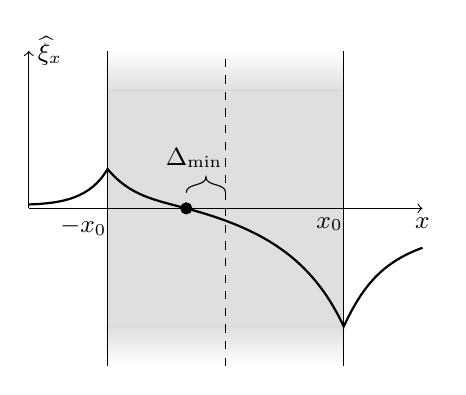
\begin{tikzpicture}
				\path [fill=lightgray, opacity=0.5] (2,-1.5) -- (2,1.5) -- (5,1.5) -- (5,-1.5) -- (2,-1.5);
				
				\shade[bottom color=white,top color=lightgray, opacity=0.5] (2,-2) to (5,-2) to (5,-1.5) to (2,-1.5) to (2,-2);
				
				\shade[top color=white,bottom color=lightgray, opacity=0.5] (2,2) to (5,2) to (5,1.5) to (2,1.5) to (2,2);
				
				\draw [-] (2,-2) -- (2,2);
				\draw [-] (5,-2) -- (5,2);
				
				%\draw [ultra thick, red, -stealth,opacity=0.7] (2.5,-1.5) -- (2.5,2);
				%\draw [ultra thick, red, path fading=south, opacity=0.5] (2.5,-2) -- (2.5,-1.5);
				%\draw [ultra thick, red, -stealth,opacity=0.7] (3,-1.5) -- (3,2);
				%\draw [ultra thick, red, path fading=south,opacity=0.5] (3,-2) -- (3,-1.5);
				%\draw [ultra thick, red, -stealth,opacity=0.7] (3.5,-1.5) -- (3.5,2);
				%\draw [ultra thick, red, path fading=south,opacity=0.5] (3.5,-2) -- (3.5,-1.5);
				%\draw [ultra thick, red, -stealth,opacity=0.7] (4,-1.5) -- (4,2);
				%\draw [ultra thick, red, path fading=south,opacity=0.5] (4,-2) -- (4,-1.5);
				%\draw [ultra thick, red, -stealth,opacity=0.7] (4.5,-1.5) -- (4.5,2);
				%\draw [ultra thick, red, path fading=south,opacity=0.5] (4.5,-2) -- (4.5,-1.5);
				
				%\draw [thick] (0,0.025) to [out=0, in=-178] (1.2, 0.05) to [out=2, in=-120] (2,0.5) to [out=-50, in=165] (3,0) to [out=-15, in=115] (5,-1.5) to [out=65, in=-170] (7,-0.2);
				
				\draw [thick] (1, 0.05) to [out=2, in=-120] (2,0.5) to [out=-50, in=165] (3,0) to [out=-15, in=115] (5,-1.5) to [out=65, in=-160] (6,-0.5);
				
				\draw [->] (1,0) -- (1,2);
				\draw [->] (1,0) -- (6,0);
				
				%\node at (1,1) {$\rho_1$};
				%\node at (6,1) {$\rho_2$};
				%\node [right] at (2.88,1.3) {$\rho_0$};
				
				\small
				\node [below left] at (2.1,0) {$-x_0$};
				\node [below left] at (5.1,0) {$x_0$};
				
				\node [right] at (1,2) {$\widehat{\xi}_x$};
				\node [below] at (6,0) {$x$};
				
				\draw [dashed] (3.5,-2) -- (3.5,2);
				\draw [fill] (3,0) circle [radius=0.07];
				\draw [-] (3, 0.2) to [out=90, in=-90] (3.25, 0.4) to [out=-90, in=90] (3.5, 0.2);
				\node [above] at (3.1, 0.4) {$\Delta_\mathrm{min}$};
				\end{tikzpicture}
			\label{fig: min pert shift saus}}
		
		
		\subfloat[]{
				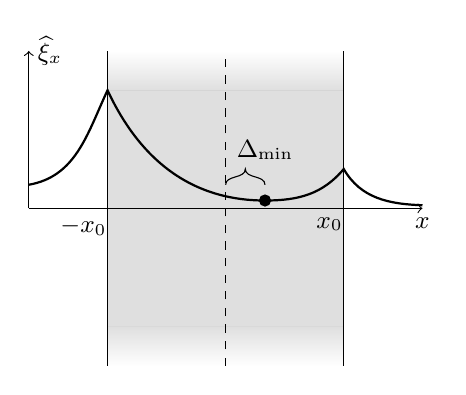
\begin{tikzpicture}
				\path [fill=lightgray, opacity=0.5] (2,-1.5) -- (2,1.5) -- (5,1.5) -- (5,-1.5) -- (2,-1.5);
				
				\shade[bottom color=white,top color=lightgray, opacity=0.5] (2,-2) to (5,-2) to (5,-1.5) to (2,-1.5) to (2,-2);
				
				\shade[top color=white,bottom color=lightgray, opacity=0.5] (2,2) to (5,2) to (5,1.5) to (2,1.5) to (2,2);
				
				\draw [-] (2,-2) -- (2,2);
				\draw [-] (5,-2) -- (5,2);
				
				%\draw [ultra thick, red, -stealth,opacity=0.7] (2.5,-1.5) -- (2.5,2);
				%\draw [ultra thick, red, path fading=south, opacity=0.5] (2.5,-2) -- (2.5,-1.5);
				%\draw [ultra thick, red, -stealth,opacity=0.7] (3,-1.5) -- (3,2);
				%\draw [ultra thick, red, path fading=south,opacity=0.5] (3,-2) -- (3,-1.5);
				%\draw [ultra thick, red, -stealth,opacity=0.7] (3.5,-1.5) -- (3.5,2);
				%\draw [ultra thick, red, path fading=south,opacity=0.5] (3.5,-2) -- (3.5,-1.5);
				%\draw [ultra thick, red, -stealth,opacity=0.7] (4,-1.5) -- (4,2);
				%\draw [ultra thick, red, path fading=south,opacity=0.5] (4,-2) -- (4,-1.5);
				%\draw [ultra thick, red, -stealth,opacity=0.7] (4.5,-1.5) -- (4.5,2);
				%\draw [ultra thick, red, path fading=south,opacity=0.5] (4.5,-2) -- (4.5,-1.5);
				
				%\draw [thick] (0,0.2) to [out=10, in=245] (2, 1.5) to [out=295, in=180] (4,0.1) to [out=0, in=230] (5,0.5) to [out=300, in=178] (6.2,0.04) to [out=358, in=180] (7,0.02);
				
				\draw [thick] (1,0.3) to [out=10, in=245] (2, 1.5) to [out=295, in=180] (4,0.1) to [out=0, in=230] (5,0.5) to [out=300, in=178] (6,0.04);
				
				\draw [->] (1,0) -- (1,2);
				\draw [->] (1,0) -- (6,0);
				%
				%\node at (1,1) {$\rho_1$};
				%\node at (6,1) {$\rho_2$};
				%\node [right] at (2.88,1.3) {$\rho_0$};
				
				\small
				\node [below left] at (2.1,0) {$-x_0$};
				\node [below left] at (5.1,0) {$x_0$};
				
				\node [right] at (1,2) {$\widehat{\xi}_x$};
				\node [below] at (6,0) {$x$};
				
				\draw [dashed] (3.5,-2) -- (3.5,2);
				\draw [fill] (4,0.1) circle [radius=0.07];
				\draw [-] (3.5, 0.3) to [out=90, in=-90] (3.75, 0.5) to [out=-90, in=90] (4, 0.3);
				\node [above] at (4, 0.5) {$\Delta_\mathrm{min}$};
				\end{tikzpicture}
			\label{fig: min pert shift kink}}}
	
	\caption{Illustration of the minimum perturbation shift, $\Delta_\textrm{min}$, within the slab (shaded) for~\protect\subref{fig: min pert shift saus}~quasi-sausage and~\protect\subref{fig: min pert shift kink}~quasi-kink modes.}
	\label{fig: min pert shift}
\end{figure}

Firstly, for quasi-sausage modes, using the solution for the transversal velocity amplitude given by Equation~\eqref{vsoln} and the expressions for the variables within given by equation~\eqref{constB C}, the minimum perturbation shift can be calculated as follows. The solution for the transversal velocity amplitude within the slab is
\begin{equation}
\widehat{v}_x(x) = B\cosh{m_0x} + C\sinh{m_0x} = 0,
\end{equation}
where $B$ is given by Equation~\eqref{constB C} and $C$ is arbitrary. This equation is solved for $x$ to give
\begin{equation}
x = \frac{1}{m_0} \tanh^{-1}\left(-\frac{B}{C}\right). \label{disp of min power saus}
\end{equation}
Therefore, the minimum perturbation shift for quasi-sausage modes is
\begin{equation}
\Delta_\textrm{min} = \frac{1}{m_0}\tanh^{-1}\left[-\frac{(k^2{v_\textrm{A}}^2 - \omega^2)m_1\frac{\rho_0}{\rho_1} - \omega^2{m_0}\tanh{m_0x_0}}{(k^2{v_\textrm{A}}^2 - \omega^2)m_1\frac{\rho_0}{\rho_1}\tanh{m_0x_0} - \omega^2{m_0}}\right]. \label{shift min saus}
\end{equation}
Similarly, for quasi-kink modes, using Equations~\eqref{vsoln} and~\eqref{constB B}, we calculate the minimum perturbation shift to be
\begin{equation}
\Delta_\textrm{min} = \frac{1}{m_0}\coth^{-1}\left(-\frac{(k^2{v_\textrm{A}}^2 - \omega^2)m_1\frac{\rho_0}{\rho_1} - \omega^2{m_0}\tanh{m_0x_0}}{(k^2{v_\textrm{A}}^2 - \omega^2)m_1\frac{\rho_0}{\rho_1}\tanh{m_0x_0} - \omega^2{m_0}}\right). \label{shift min kink}
\end{equation}
The dependence of the minimum perturbation shifts on the external plasma region with subscript~2 is implicit in the determination of the eigenfrequency $\omega$ when solving the dispersion relation.

The concept of minimum perturbation shift is exclusive to surface modes. The eigenfunctions of surface modes in a magnetic slab are significantly more sensitive to the external plasma parameters than body modes \citep{all_etal17}. This makes intuitive sense given that the energy in a surface mode is localised to the boundaries of the slab whereas the energy in a body mode is largely isolated within the slab. There is a shift in the spatial nodes and anti-nodes in body mode perturbations within a slab due to changing external plasma parameters, however, it is too small to be an effective observational tool.

Akin to the amplitude ratio method for solar magneto-seismology prescribed in Section~\ref{sec: AR}, we can invert Equation~\eqref{shift min saus} or~\eqref{shift min kink} for the the Alfv\'{e}n speed, $v_\textrm{A}$, and hence get an estimate the magnetic field strength of inhomogeneous solar magnetic structures. This can be done either numerically, using an iterative root finding method, or analytically, under an appropriate approximation. In each of the following subsections, we discuss the analytical inversion procedure under the thin slab (Section~\ref{sec: mps thin}), wide slab (Section~\ref{sec: mps wide}), incompressible (Section~\ref{sec: mps incomp}), and low-beta (Section~\ref{sec: mps low-beta}) approximations.


\subsection{Thin slab approximation} \label{sec: MPS thin}
Under the thin slab approximation, that is $kx_0 \ll 1$, we have $m_0x_0 \ll 1$ for surface modes (Section~\ref{sec: thin slab}). By definition, $|\Delta_\textrm{min}| < x_0$, therefore, $m_0|\Delta_\textrm{min}| \ll 1$, so that $\tanh{m_0\Delta_\textrm{min}} \approx m_0\Delta_\textrm{min}$. Firstly, for quasi-sausage modes in a thin slab, Equation~\eqref{shift min saus} can be solved for $v_\textrm{A}$ to give
\begin{equation}
v_\textrm{A}^2 = \frac{\omega^2}{k^2} \left[\frac{\rho_1}{\rho_0m_1}(x_0 + \Delta_\textrm{min}) + \frac{1}{1 + (\omega / kc_0)^2} + k^2x_0\Delta_\textrm{min}\right].
\end{equation}
For quasi-kink modes in a thin slab, Equation~\eqref{shift min kink} can be solved for $v_\textrm{A}$ to give
\begin{equation}
v_\textrm{A}^2 = \frac{\omega^2}{k^2}\left[\frac{-b \pm \sqrt{b^2 - 4ac}}{2a}\right],
\end{equation}
where
\begin{align}
a &= m_1\frac{\rho_0}{\rho_1}(k^2c_0^2 - \omega^2)(x_0 + \Delta_\textrm{min}), \\
b &= -m_1\frac{\rho_0}{\rho_1}(2k^2c_0^2 - \omega^2)(x_0 + \Delta_\textrm{min}) - (k^2c_0^2 - \omega^2), \\
c &= c_0^2m_1\frac{\rho_0}{\rho_1}(x_0 + \Delta_\textrm{min}) + c_0^2 + \omega^2x_0\Delta_\textrm{min}.
\end{align}


\subsection{Wide slab approximation} \label{sec: mps wide}
The concept of minimum perturbation shift is ill-defined under the wide slab approximation, that is, when $kx_0 \gg 1$. In this case, each interface oscillates independently at its own eigenfrequency. Therefore the nomenclature of quasi-sausage and quasi-kink mode breaks down. In the wide slab limit, the eigenfunctions have no local minimum in the slab, instead the perturbations are evanescent away from the oscillating interface, therefore there is no local minimum of wave power within the slab.


\subsection{Incompressible approximation} \label{sec: mps incomp}
When the plasma is incompressible, the sound speeds are unbounded, so that $m_j = k$, for $j = 0, 1, 2$. The minimum perturbation shift for a quasi-sausage mode (top) and quasi-kink (bottom) in an incompressible slab is
\begin{equation}
\Delta_\textrm{min} = \frac{1}{k}\left(\begin{matrix} \tanh^{-1} \\ \coth^{-1} \end{matrix}\right)\left(-\frac{(k^2{v_\textrm{A}}^2-\omega^2)\frac{\rho_0}{\rho_1} - \omega^2\tanh{kx_0}}{(k^2{v_\textrm{A}}^2-\omega^2)\frac{\rho_0}{\rho_1}\tanh{kx_0} - \omega^2}\right),
\end{equation}
which can be solved for $v_\textrm{A}$ to give
\begin{equation}
v_\textrm{A}^2 = \frac{\omega^2}{k^2}\left[1 + \frac{\rho_1}{\rho_0}\left(\begin{matrix} \tanh \\ \coth \end{matrix}\right)(k(x_0 + \Delta_\textrm{min}))\right].
\end{equation}


\subsection{Low-beta approximation} \label{sec: mps low-beta}
In a low-beta plasma, the minimum perturbation shift for a quasi-sausage mode (top) and quasi-kink (bottom) is given by
\begin{equation}
\Delta_\textrm{min} = \frac{1}{k}\left(\begin{matrix} \tanh^{-1} \\ \coth^{-1} \end{matrix}\right)\left(-\frac{(k^2{v_\textrm{A}}^2 - \omega^2)m_1\frac{\rho_0}{\rho_1} - \omega^2k\tanh{kx_0}}{(k^2{v_\textrm{A}}^2 - \omega^2)m_1\frac{\rho_0}{\rho_1}\tanh{kx_0} - \omega^2k}\right),
\end{equation}
which can be solved for $v_\textrm{A}$ to give
\begin{equation}
v_\textrm{A}^2 = \frac{\omega^2}{k^2}\left[1 + \frac{k\rho_1}{m_1\rho_0}\left(\begin{matrix} \tanh \\ \coth \end{matrix}\right)(k(x_0 + \Delta_\textrm{min}))\right].
\end{equation}


\begin{sidewaystable}
	\centering
	\begin{tabular}{lccc}
		\toprule
		\smallskip
		Mode & \multicolumn{3}{c}{Approximation of $k^2v_\textrm{A}^2 / \omega^2$ using the amplitude ratio, $R_\textrm{A}$} \\
		& Thin slab & Incompressible & Low-beta \\
		\midrule
		\smallskip
		Quasi-sausage surface & $ 1 + \frac{1}{x_0}\left(\frac{R_\textrm{A}\frac{\rho_2}{\rho_0m_2} + \frac{\rho_1}{\rho_0m_1}}{R_\textrm{A} + 1}\right) $ & $ 1 + \left( \frac{R_\textrm{A} \frac{\rho_2}{\rho_0} + \frac{\rho_1}{\rho_0}}{R_\textrm{A} + 1} \right) \coth{kx_0} $ & $ 1 + k \left( \frac{ R_\textrm{A}\frac{\rho_2}{\rho_0m_2} + \frac{\rho_1}{\rho_0m_1}}{R_\textrm{A} + 1} \right) \coth{kx_0} $ \\
		Quasi-kink surface & $ 1 + k^2x_0\left(\frac{R_\textrm{A}\frac{\rho_2}{\rho_0m_2} - \frac{\rho_1}{\rho_0m_1}}{R_\textrm{A} - 1}\right) $ & $ 1 + \left( \frac{R_\textrm{A} \frac{\rho_2}{\rho_0} - \frac{\rho_1}{\rho_0}}{R_\textrm{A} - 1} \right) \tanh{kx_0} $ & $ 1 + k \left( \frac{ R_\textrm{A}\frac{\rho_2}{\rho_0m_2} - \frac{\rho_1}{\rho_0m_1}}{R_\textrm{A} - 1} \right) \tanh{kx_0} $ \\
		\bottomrule
	\end{tabular}
	\caption{Magneto-seismology inversion using the amplitude ratio, $R_\textrm{A}$, to approximate the Alfv\'{e}n speed, $v_\textrm{A}$.}
	\label{table: amp ratio}

	\bigskip\bigskip\bigskip\bigskip\bigskip

	\begin{tabular}{lccc}
		\toprule
		\smallskip
		Mode & \multicolumn{3}{c}{Approximation of $k^2v_\textrm{A}^2 / \omega^2$ using the minimum perturbation shift, $\Delta_\textrm{min}$} \\
		& Thin slab & Incompressible & Low-beta \\
		\midrule
		\smallskip
		Quasi-sausage surface & $ \frac{\rho_1}{\rho_0m_1}(x_0 + \Delta_\textrm{min}) + \frac{1}{1 + (\omega / kc_0)^2} + k^2x_0\Delta_\textrm{min} $ & $ 1 + \frac{\rho_1}{\rho_0}\tanh{k(x_0 + \Delta_\textrm{min})} $ & $ 1 + \frac{k\rho_1}{m_1\rho_0}\tanh{k(x_0 + \Delta_\textrm{min})} $ \\
		Quasi-kink surface & $\frac{-b \pm \sqrt{b^2 - 4ac}}{2a}$, defined in Section~\ref{sec: mps thin} & $ 1 + \frac{\rho_1}{\rho_0}\coth{k(x_0 + \Delta_\textrm{min})} $ & $ 1 + \frac{k\rho_1}{m_1\rho_0}\coth{k(x_0 + \Delta_\textrm{min})} $ \\
		\bottomrule		
	\end{tabular}
	\caption{Magneto-seismology inversion using the minimum perturbation shift, $\Delta_\textrm{min}$, to approximate the Alfv\'{e}n speed, $v_\textrm{A}$.}
	\label{table: min pert shift}
\end{sidewaystable}


%------------------------------------------------------------------------------
\section{Numerical inversion procedure}
\label{sec: numerical inversion}
%------------------------------------------------------------------------------

We have introduced the amplitude ratio and the minimum perturbation shift which quantify the spatial asymmetry in magnetic slab eigenmodes. These expressions can be applied to determine the Alfv\'{e}n speed, for a given set of observed equilibrium parameters, providing us a novel method to diagnose information about the background plasma, thus advancing the field of spatial magneto-seismology.

A summary of the analytical expressions for estimating the Alfv\'{e}n speed, $v_\textrm{A}$, within an asymmetric magnetic slab is given in Tables~\ref{table: amp ratio} and~\ref{table: min pert shift}, utilising the amplitude ratio method and the minimum perturbation shift method, respectively. With these analytical inversions, theoretical simplicity comes at the cost of having to use an additional approximation.

A second option is to solve the inverse problem numerically. In practice, a numerical procedure could be made relatively simple and computationally inexpensive by making use of a standard root finding method once the observed parameters have been prescribed.


\subsubsection{Estimating a single parameter} \label{sec: single param}

The diagnosis procedure for one background parameter - the Alfv\'{e}n speed, for example - is as follows:
\begin{enumerate}
	\item Observe an oscillating asymmetric MHD waveguide in the solar atmosphere.
	\item Decompose into asymmetric MHD wave modes.
	\item Measure wave parameters: angular frequency and wavelength.
	\item Measure background parameters: waveguide width, density, and temperature (and hence sound speed).
	\item Measure a diagnostic parameter: amplitude ratio or minimum perturbation shift.
	\item Use a root-finding technique to solve the diagnostic equation (Equation~\eqref{AR saus}, \eqref{AR kink}, \eqref{shift min saus}, or~\eqref{shift min kink}, depending on the mode identified and the diagnostic parameter used) for the Alfv\'{e}n speed.
\end{enumerate}
In practice, Step~3 us often extremely difficult. In addition to the Alfv\'{e}n speed, the density across the waveguide is very difficult to measure \citep{war_etal09}. One way around this is to estimate multiple parameters simultaneously, as discussed in Section~\ref{sec: multiple params}.

Figure~\ref{fig: AR MPS} illustrates the dependency of the amplitude ratio and minimum perturbation shift on the (non-dimensionalised half) slab width, $kx_0$, and the density ratio, $\rho_1/\rho_0$, of one external plasma density to the slab density, holding the other external density fixed. Varying one density ratio in this way is equivalent to changing the degree of asymmetry of the waveguide. The amplitude ratio is positive (negative) for quasi-kink (quasi-sausage) modes, because the oscillations on each boundary are in phase (anti-phase). Figures~\ref{fig: AR slow kink surf} and~\ref{fig: AR slow saus surf} further show that, for a given background parameter regime, the boundary with the highest amplitude is different for quasi-kink and quasi-sausage modes. This is demonstrated by the absolute value of the amplitude ratio being greater than 1 for quasi-sausage modes when it is less than 1 for quasi-kink modes, and \textit{vice versa}. This is in agreement with the properties of the eigenmodes of the analogous spring-mass system introduced by \cite{all_etal17} and discussed in Section~\ref{sec: mechanical analogy}. Figures~\ref{fig: MPS slow kink surf} and~\ref{fig: MPS slow saus surf} demonstrate that the position of minimum perturbation for quasi-kink modes is shifted in the opposite direction to that of quasi-sausage modes.

\begin{figure}
	\centering
	\subfloat[Quasi-kink]{\includegraphics[width=0.5\textwidth]{\figdirV slow-kink-surf_amp-ratio.pdf}
		\label{fig: AR slow kink surf}}
	\subfloat[Quasi-sausage]{\includegraphics[width=0.5\textwidth]{\figdirV slow-saus-surf_amp-ratio.pdf}
		\label{fig: AR slow saus surf}}
	\\
	\subfloat[Quasi-kink]{\includegraphics[width=0.5\textwidth]{\figdirV slow-kink-surf_min-pert-shift.pdf}
		\label{fig: MPS slow kink surf}}
	\subfloat[Quasi-sausage]{\includegraphics[width=0.5\textwidth]{\figdirV slow-saus-surf_min-pert-shift.pdf}
		\label{fig: MPS slow saus surf}}
	\caption{(\protect\subref*{fig: AR slow kink surf}, \protect\subref*{fig: AR slow saus surf}) The amplitude ratio, $R_\textrm{A}$, and (\protect\subref*{fig: MPS slow kink surf}, \protect\subref*{fig: MPS slow saus surf}) the minimum perturbation shift, $\Delta_\textrm{min}$, as a function of the slab width, non-dimensionalised to $kx_0$, and the density ratio, $\rho_1/\rho_0$, for slow (\protect\subref*{fig: AR slow kink surf}, \protect\subref*{fig: MPS slow kink surf}) quasi-kink and (\protect\subref*{fig: AR slow saus surf}, \protect\subref*{fig: MPS slow saus surf}) quasi-sausage surface modes. The other density ratio is set to $\rho_2/\rho_0 = 2$, the characteristic speed ordering inside the slab is $v_\textrm{A}=1.3c_0$, and the sound speed outside the slab is determined to ensure equilibrium pressure balance.}
	\label{fig: AR MPS}
\end{figure}


\subsubsection{Estimating multiple parameters} \label{sec: multiple params}

It is often the case that not all the non-magnetic parameters characterising a waveguide are well-observable. In particular, the density distribution across the waveguide is, like the Alfv\'{e}n speed, often impossible to determine. Thankfully, a combination of the amplitude ratio method and minimum perturbation shift method can be employed to diagnose multiple unknown background parameters. Using a combination of observables to be able to estimate multiple background parameters has been explored by \cite{arr_etal07,Goo_etal08}.

The motivation for this combined technique is as follows. The dispersion relation, the amplitude ratio method, and minimum perturbation shift method give us a set of three functions where the zeros of each function correspond to solutions of the respective equation. Denoting the wave parameters and background parameters by $p_\mathrm{w}$ and $p_\mathrm{bg}$, respectively, these functions (for a quasi-sausage mode) are
\begin{align}
D(p_\mathrm{w}, p_\mathrm{bg}) &= (\Lambda_0c_0 + \Lambda_2s_0)(\Lambda_0s_0 + \Lambda_1c_0) + (\Lambda_0c_0 + \Lambda_1s_0)(\Lambda_0s_0 + \Lambda_2c_0), \label{disp func} \\
f_{\mathrm{AR}}(R_\mathrm{A}, p_\mathrm{w}, p_\mathrm{bg}) &= R_A + \frac{\rho_1m_2}{\rho_2m_1}\left[\frac{(k^2v_\textrm{A}^2 - \omega^2)m_1\frac{\rho_0}{\rho_1} - \omega^2m_0\coth{m_0x_0}}{(k^2v_\textrm{A}^2 - \omega^2)m_2\frac{\rho_0}{\rho_2} - \omega^2m_0\coth{m_0x_0}}\right], \label{AR func} \\
f_{\mathrm{MPS}}(\Delta_\mathrm{min}, p_\mathrm{w}, p_\mathrm{bg}) &= \Delta_\textrm{min} - \frac{1}{m_0}\tanh^{-1}\left[-\frac{(k^2{v_\textrm{A}}^2 - \omega^2)m_1\frac{\rho_0}{\rho_1} - \omega^2{m_0}\tanh{m_0x_0}}{(k^2{v_\textrm{A}}^2 - \omega^2)m_1\frac{\rho_0}{\rho_1}\tanh{m_0x_0} - \omega^2{m_0}}\right]. \label{MPS func} \\
\end{align}
The zeros of each of these functions correspond to solutions of Equations~\eqref{disp rel}, \eqref{AR saus}, and~\eqref{shift min saus}. The single parameter estimation involves using a single-variable root-finding scheme (such as the secant method) to find the zeros of either $f_\mathrm{AR}$ or $f_\mathrm{MPS}$, depending on whether the diagnostic parameter is the amplitude ratio or the minimum perturbation shift (see Section~\ref{sec: single param}). Alternatively, notice that setting Equations~\eqref{disp func}-\eqref{MPS func} to zero forms a system of three coupled equations. Therefore, given measurements of one or two diagnostic parameters, $R_\mathrm{A}$ or $\Delta_\mathrm{min}$, all but up to three background parameters, $p_\mathrm{bg}$, we can use a multivariate root-finding algorithm to solve up to three of these equations. Effectively, the extra diagnostic parameter and the dispersion relation each reduce the number of degrees of freedom. Thus, we can estimate up to three parameters.

As an example, the procedure to estimate the Alfv\'{e}n speed and both the density ratios is as follows:
\begin{enumerate}
	\item Observe an oscillating asymmetric MHD waveguide in the solar atmosphere.
	\item Decompose into asymmetric MHD wave modes.
	\item Measure wave parameters: angular frequency and wavelength.
	\item Measure background parameters: waveguide width and temperature (and hence sound speed).
	\item Measure diagnostic parameters: amplitude ratio and minimum perturbation shift.
	\item Use a multi-variate root-finding algorithm to find the values of the Alfv\'{e}n speed and the two density ratios for which the functions~\eqref{disp func}-\eqref{MPS func} are zero.
\end{enumerate}

As an example, Figure~\ref{fig: vA approx} shows the inversion curves for a particular parameter regime typical of a slow surface mode. It is plotted by prescribing (as if they were observed quantities) all plasma parameters except the Alfv\'{e}n speed, $v_\textrm{A}$, and one of the density ratios, $\rho_1/\rho_0$, then simultaneously solving the dispersion relation, Equation~\eqref{disp rel}, with the equations for the amplitude ratio, Equation~\eqref{AR saus} or~\eqref{AR kink}, or the minimum perturbation shift, Equation~\eqref{shift min saus} or~\eqref{shift min kink}. The solution curves were calculated numerically using Powell's Method, which is an efficient algorithm for calculating the minimum of a multivariate function when the partial derivatives are not available analytically \citep{pow64}.

\begin{figure}
	\centering
	\subfloat[Amplitude ratio inversion]{\includegraphics[scale=0.5]{\figdirV RA_vA_approx_2var.pdf}
		\label{fig: RA vA approx}} \\
	\subfloat[Minimum perturbation shift inversion]{\includegraphics[scale=0.5]{\figdirV DM_vA_approx_2var.pdf}
		\label{fig: DM vA approx}}
	\caption{Using prescribed values for~\protect\subref{fig: RA vA approx}~the amplitude ratio, $R_\textrm{A}$, or~\protect\subref{fig: DM vA approx}~the minimum perturbation shift, $\Delta_\textrm{min}$, a numerical inversion is used to approximate the background equilibrium parameters, in this case the Alfv\'{e}n speed, $v_\textrm{A}$, and one of the density ratios, $\rho_1 / \rho_0$, for slow magneto-acoustic modes. Dashed (solid) lines correspond to the inversion curves for slow quasi-kink (quasi-sausage) surface modes. The dotted lines indicate the inversion for symmetric kink and sausage modes. The light-shaded area indicates the values of the Alfv\'{e}n speed which correspond to body modes, rather than surface modes, so are not important for SMS application. The dark shaded region in Figure~\protect\subref{fig: DM vA approx} illustrates the region outside the slab, outside the bounds of the minimum perturbation shift.}
	\label{fig: vA approx}
\end{figure}

The ability to diagnose multiple parameters simultaneously could in some cases get around the hurdle of uncertain density measurements. However, the cost of this is that by estimating several parameters, we are more likely to encounter multiple roots (Section~\ref{sec: multiple roots}).


\subsubsection{Error analysis}

Every measurement comes with error, and when assessing the efficacy of a new measurement technique, an analysis of the errors must be undertaken. There are two kinds of error in a diagnosis made using the AR and MPS methods: \textit{propagated errors} that are due to errors in them measurement of the input parameters, and \textit{systematic errors} that are due to the asymmetric waveguide model approximating the real structure less than perfectly.

To analyse the propagated error, we determine which input parameters are most uncertain and hence are likely to contribute the most uncertainty to the diagnosed parameters. When density is used as an input parameter, it is often the case that the error in its measurement dominates the errors in all other input parameters. Errors in spatial parameters, such as the waveguide width, and temporal parameters, such as the angular frequency, are generally much smaller. The propagation of the error in the density is reduced by a factor of two by the square root that is introduced when inverting $v_A$ from $k^2v_A^2/\omega^2$ (in a similar way to \citealp{nak_etal01}). That is, a relative error of 10\% in the density leads to a relative error of approximately 5\% in the Alfv\'{e}n speed estimation. Furthermore, with high precision methods using density-sensitive emission lines \citep{you_etal09}, the propagation of density measurement errors can be reduced.

As we have seen in Section~\ref{sec: multiple params}, the density need not be an input parameter if both the amplitude ratio and the minimum perturbation shift are observable. In this case, I expect that the input parameter with the highest uncertainty would be the minimum perturbation shift. This is because . Nevertheless, in the same way as the error in density, the relative error in the measurement of the minimum perturbation shift reduces by a factor of two when propagated through to the relative uncertainty in the estimated parameters.

The systematic error is more difficult to analyse quantitatively. The main sources of systematic error include:
\begin{enumerate}
	\item The waveguide is not well-modelled as an asymmetric slab, \label{not slab}
	\item The wave is significantly nonlinear, \label{nonlinear}
	\item The wrong solution is found to the parameter inversion. \label{wrong solution}
\end{enumerate}
Error sources \ref{not slab} and~\ref{wrong solution} are discussed in Sections~\ref{sec: SMS discussion} and~\ref{sec: multiple roots}, respectively. Regarding error source~\ref{nonlinear}, unfortunately, a thorough study into the effects of MHD wave nonlinearity on seismology inversions is yet to be conducted. For this reason, it is unclear to what extent neglecting nonlinearity contributes to the errors in the present seismological inversion.


\subsubsection{Dealing with multiple solutions} \label{sec: multiple roots}

A common pitfall when solving inverse problems is identifying the \textit{wrong} solution\footnote{The \textit{wrong} solutions are not wrong in the sense that they don't mathematically solve the equations, rather they are wrong in the sense that they do not map to reality.}. Even the most simple functions can have a multivalued inverse. For example, the function $f(x) = x^2$ has inverse function $f^{-1}(x) = \sqrt{x}$, which is multivalued, for example, $f^{-1}(1) = 1$ or $-1$. If we were looking specifically for the solution $1$ but found only the solution $-1$, we'd have found the \textit{wrong} solution. The original function does not preserve the complete information of the input, so there is no way of getting the missing information when given only the output.

Solar magneto-seismology techniques can lead to problems of a multivalued inverse. In theory, there can be multiple values of the background parameters that will lead to a given observational signature of MHD waves. Therefore, given only the observational signature, is not always possible to find an unambiguous solution to the inverse problem. Sometimes we cannot be sure that our estimation of the background parameters is the correct one, leading to significant systematic error. This problem is more likely to raise its head when attempting to estimate multiple background parameters, such as described in Section~\ref{sec: multiple params}. This is due to there being more dimensions over which the original function can be non-injective. Non-injectivity of the original function is sufficient to guarantee that its inverse function is multivalued. It is even possible for there to be infinitely many solutions to the seismological inverse problems that are all equally likely.

One way around the problem of the multivalued inverse is to use prior information about the MHD waveguide to inform our choice of the correct solution. This is the domain of Bayesian statistics \citep{arr_etal11,arr_etal18}. Bayesian statistics can provide a mathematically precise formulation of multivalued inverse problems in probabilistic terms. It can be used to determine which seismological solution is \textit{more likely} to be correct. For example, let's say we are solving an inverse problem to estimate the magnetic field strength in a quiescent prominence. If we lived in a world where we knew nothing at all about the conditions in a prominence, we would have no way to preference one solution to the inverse problem over another. However, we do not live in that world. Based on several decades worth of of solar observations from tens of solar observatories, we have prior understanding of the range of parameter values we'd expect to observe. We would be more surprised to find a value of 0.01~Gauss or 1000~Gauss than we would be for a value of, say, 10~Gauss. Bayesian statistic formalises this probabilistic reasoning. The posterior distribution gives the \textit{degree of belief} of the parameter of interest.

As well as helping to determine which parameter values are more likely to be correct, Bayesian statistics can be useful for model comparison \citep{arr_etal18}. This is a method of quantitatively assessing which of several models is favoured by the data. It provides a well defined degree of belief in each of the models. This is a promising way to reduce the systematic error in seismological inversions. We note both Bayesian inversion and Bayesian model comparison as promising topics for future study in Chapter~\ref{chap: future work}.


\subsubsection{Sensitivity to input parameters}

The amplitude ratio has a strong sensitivity to the changes in the external densities, and therefore the external asymmetry, whereas the minimum perturbation shift has a weaker dependency. Therefore, the amplitude ratio is likely to be a more effective parameter for diagnosing background parameters. Furthermore, observations of the location of the minimum wave power within a solar magnetic slab will be fraught with noise, potentially causing the detection of a false minimum. Noise in amplitude ratio measurements is less likely to introduce large errors because the locations of the slab boundaries are a more obvious features and can be identified by the steep gradients in the wavelength of observed light, for example, and is stable to larger noise signals.

Both the amplitude ratio and minimum perturbation shift are more sensitive to small changes in the background equilibrium parameters, \emph{i.e.} the asymmetry in the background plasma, than the eigenfrequencies are. On a theoretical level, this corroborates with the result that eigenfunctions of linear operators on a Hilbert space are often more sensitive to small perturbations of the operator than their corresponding eigenvalues \citep{kat95}. The amplitude ratio and minimum perturbation shift parameters depend on the eigenfunctions, $\widehat{v}_x(x)$, as well as the eigenvalues, $\omega^2$. This means that spatial seismology techniques can be theoretically more effective than temporal techniques for many solar structure. Therefore, we are excited to see a push for increased spatial resolution with next-generational observational instrumentation such as the Daniel K. Inouye Solar Telescope (DKIST). Upon completion, this will equip us to be able to use the magneto-seismology techniques developed here to better understand the diagnostic properties of asymmetric slab-like solar atmospheric structures such as elongated magnetic bright points, prominences, and sunspot light walls.


%------------------------------------------------------------------------------
\section{Discussion of the application of these techniques}
\label{sec: SMS discussion}
%------------------------------------------------------------------------------

The Amplitude Ratio Method and Minimum Perturbation Shift Method present interesting and novel approaches to solar magneto-seismology. Their application is appropriate only to solar atmospheric waveguides that approximate the slab waveguide model. The simplicity of the model used to derive these techniques means that we are restricted in their application. In this section, we outline several solar atmospheric structures that could lend themselves to analysis by the seismological methods introduced in this thesis, namely, chromospheric fibrils, magnetic bright points, quiescent prominences, and light walls.



Large magnetic bright points (MBPs), with characteristic length $L > 500$ km, along inter-granular lanes are often rather elongated \citep{cro_etal10}. The application of SMS techniques to MBPs is limited by the low spatial resolution of current observations. DKIST is going to have a spatial resolution of 19 km for structures on the solar surface \citep{tri_etal15}, sufficient enough to resolve oscillations in MBPs. This unprecedented resolution will hopefully give the sufficient number of pixels (5-10) across an MBP to determine whether their oscillations have maximum power at the boundaries of or within the waveguide, that is, to differentiate between the transverse eigenfunctions of surface and body MHD modes, respectively. This is crucial for the accurate employment of these SMS techniques, and would build upon previous work on mode identification such as the surface modes that were identified in photospheric pores \citep{mor_etal15}.

Quiescent prominences, which are large long-lived magnetic formations of cool dense plasma elevated into the hot and rarefied coronal atmosphere, can be approximated by magnetic slabs and have been regularly observed to guide MHD waves \citep{arr_etal12}. The basic slab model of prominences, as illustrated by \textit{e.g.} \cite{joa_etal92a,joa_etal92b}, is of a symmetric slab, however, a small asymmetry could easily be caused by adjacent inhomogeneities. Even a small asymmetry in density ($|1 - \rho_1/\rho_2| < 0.1$) can cause a significant (factor of 2 or more) asymmetry in the eigenmode (Figure~\ref{fig: AR MPS}), except for in thin slabs. This makes prominences a good candidate for applying the SMS techniques developed here. One issue that one has to bear in mind for the employment of these techniques is that the approximation of simple asymmetric magnetic slab may be insufficient to capture some important aspects of prominence oscillations, in particular, prominences are likely to have a sheared magnetic field and may have significant flows, which are neglected in the asymmetric slab model \citep{van_etal89,zir_etal94,bal05,oli09,arr_etal12}.

Light bridge surges also present a possible application. Rooted in sunspot light bridges, these clusters of recurrent chromospheric surges observed as bright structures in \textit{e.g.} IRIS 1330~\AA~line, as observed by \cite{yan_etal16} are formed by either magnetic reconnection just above the light bridge \citep{tor_etal15,rob_etal16} or by leakage of p-modes from beneath the underlying photosphere \citep{yan_etal15,zha_etal17}. They have been demonstrated to guide MHD waves driven by nearby disturbances \citep{yan_etal16,yan_etal17}. While the asymmetric magnetic slab could be a valid approximation for the actual geometry of light walls, the strong magnetic field in the low solar atmosphere above a sunspot umbra (the plasma each side of the light bridge) may put into question the full validity of the non-magnetic external plasma in the current model. However, what matters is the relative strength of the magnetic force compared to the pressure gradient force, that is, the value of plasma-beta. The value of beta above magnetic pores and sunspots is uncertain, but has been shown to be rather high in some cases \citep{bou17}, and has therefore been used in models of the low atmosphere \citep{mum_etal15}. With improved observations, it may turn out that the plasma surrounding light walls has a low-beta, in which case, we suggest that a future generalisation of the methods described here which involves an asymmetric magnetic plasma outside the slab will be a more appropriate method for the first magneto-seismology diagnosis of sunspot light walls.

Of course, these methods have limits of applicability due to the fact that we have modelled the slab as infinitely long, yet there do not exist any infinitely long waveguides in the solar atmosphere. However, if the length, $L$, of the cross section of an observed solar waveguide is much greater than its width, $x_0$, say $L/x_0 = 5-10$, then this model of an infinitely long slab may be a valid approximation. Furthermore, if the wavelength of the observed wave, $\lambda$, is such that $L \gg \lambda \gg x_0$, then the thin slab approximation holds (Sections~\ref{sec: AR thin slab} and~\ref{sec: MPS thin}), therefore an analytical diagnosis of the Alfv\'{e}n speed within the waveguide can be made using Table~\ref{table: amp ratio} or~\ref{table: min pert shift}.


\subsubsection{Possible alternative causes of asymmetry}

As a word of warning before we demonstrate a first use of these new SMS techniques, the observed asymmetry of solar MHD waves may not always be a consequence of underlying asymmetry in the background plasma. There are three mechanisms other than asymmetry in the equilibrium plasma that can plausibly explain observed asymmetry of MHD waves:
\begin{enumerate}
	\item Local oscillations,
	\item Collective oscillations of a larger waveguide,
	\item Multiple overlying oscillating waveguides.
\end{enumerate}
In the following paragraphs, we explain the mechanism and discuss their plausibility as alternative hypotheses.

The first alternative possibility is that when we observe asymmetry in MHD waves, we are actually observing a symmetric MHD structure that is oscillating locally rather than as a whole. The eigenmodes described in Section~\ref{sec: EVP} are oscillations of the waveguide as a whole. This type of oscillation is known as a \textit{collective} or \textit{global} oscillation. If the waveguide's characteristic length-scale (which is equal to the slab width for a magnetic slab) is much greater than the wave's characteristic length-scale, then a portion of the structure can oscillate without perturbing the rest of the structure. For example, each interface of a symmetric slab can oscillate independently with a wave whose wavelength is much shorter than the slab width\footnote{this was shown analytically in Section~\ref{sec: wide slab}.}. Two parallel interfaces oscillating independently with different amplitudes could be erroneously interpreted as a collective asymmetric oscillation of the whole waveguide. It is unclear how likely this hypothesis is to be true over the hypothesis of asymmetric equilibrium parameters.

Secondly, the structure that appears to be oscillating asymmetrically could be oscillation as part of a larger structure. For example, a symmetric magnetic slab or axisymmetric flux tube could oscillate collectively with several adjacent structures to form a larger scale asymmetric waveguide (as studied by \cite{shu_etal18} for a slab as part of a larger system of several parallel interfaces and by \cite{van_etal08} for a flux tube oscillating with an adjacent flux tube). It is conceivable that if part of the larger waveguide is obfuscated from view, that the symmetric visible part (say, a structure approximating a symmetric slab or axisymmetric flux tube) is oscillating asymmetrically. This seems highly unlikely to explain many asymmetric waves observation due to the improbability of the equilibrium set-up.

A third alternative possibility to explain the observed asymmetry is that we are observing several overlying structures. When observing in a optically thin spectral line, each pixel is made up of the integral of light emitted by plasma along the line-of-sight. For example, an observation of the chromosphere made with the commonly used H$\alpha$ emission line is made up of a light emitted from the multiple overlying structures between the telescope and the optically thick photosphere. It is impossible to isolate how much each structure contributes to the emission\footnote{With multiple telescopes observing the same point in three-dimensional space but from different angles, we can get much closer to isolating the light emission from a single structure. This is the project of the Stereo mission \citep{stereo}.}. For this reason, observed asymmetry of an MHD wave could be due to several overlying structures moving in a way that appears like a single asymmetric oscillation. That is, it could be an observational artefact due to the optically thin plasma rather than due to asymmetry in the equilibrium structure. This strikes us as an implausible mechanism. This is because the combination of emission from overlying structures would be far more likely to combine into an incoherent oscillation in the optically thin line. For example, in the chromospheric H$\alpha$ data analysed in Section~\ref{sec: data}, most of the observational domain is a sea of incoherently oscillating fibrils. We identify this as being due to overlying structures obscuring coherently oscillating waveguide. We also see many structures oscillating coherently for several periods, all of which demonstrate some degree of asymmetry. Were this asymmetry due to overlying structures, we would expect them to not oscillate coherently for as long, and to be much smaller in number. Therefore, we reject this possibility.


%------------------------------------------------------------------------------
\section{Diagnosing the Alfv\'{e}n speed of chromospheric fibrils}
\label{sec: fibrils}
%------------------------------------------------------------------------------

The Alfv\'{e}n speed in the chromospheric quiet Sun is highly inhomogeneous, due to the many magnetic structures that make up the magnetic canopy, and undergoes a steep gradient from $15~\text{km~s}^{-1}$ in photospheric flux tubes to $1000~\text{km~s}^{-1}$ in the corona \citep{van_etal11}. The Alfv\'{e}n speed in specific chromospheric structures is very hard to determine using current techniques. At best, we can use extrapolations from the photospheric magnetic field, but since the chromosperic magnetic field is non-potential \citep{woo_etal99,wie_etal14}, the errors are significant.
In this section, we apply the Amplitude Ratio Method to make an estimate of the Alfv\'{e}n speed in several chromospheric fibrils.


\subsection{Data} \label{sec: data}

The data were taken from observations close to the disk centre with a narrow-band 0.25 \AA~H$\alpha$ core (6562.8~\AA) filter on the 29th September 2010 using the Rapid Oscillations in the Solar Atmosphere (ROSA) imager on the Dunn Solar Telescope \citep{jes_etal10a}. The data show a dynamic sea of dark dense fibrils that map, at least partially, the inter-network magnetic field overlying the bright and less dense plasma that permeates the quiet Sun \citep{lee_etal12}. The implementation of the Amplitude Ratio Method involves resolving sub-fibril structure, for which the ROSA instrument’s high spatial (150~km) and temporal resolution (7.68~s) were just barely sufficient, with 10-20~pixels (width $\sim$50~km) across each fibril.

More information about the observations is detailed by \cite{mor_etal12}, who originally used the same data for the analysis of ubiquitous MHD waves in the chromosphere. They interpreted the observed fibril oscillations as concurrent sausage and kink modes of circular cross-sectional magnetic flux-tubes. In the present analysis, we propose an alternative interpretation that the oscillations are MHD oscillations in asymmetric waveguides. The strong phase relationship between and the similar phase speeds measured for the oscillations in each of the transverse axial displacement, the cross-sectional width, and the integrated intensity across the fibrils (see \citealp{mor_etal12}), is some evidence for the present interpretation. However, we wish to make it clear that this interpretation is taken mainly to \textit{demonstrate} a new SMS technique which depends on the existence of waveguide asymmetry. The evidence for or against either interpretation (concurrent modes in symmetric waveguides or individual modes in asymmetric waveguides) is too weak to be conclusive.


\subsection{Methodology}

In the absence of MHD wave theory in more realistic asymmetric geometries, we model each fibril as an isolated magnetic slab whose boundaries are parallel discontinuities between the uniform internal plasma and the asymmetric external plasma (Figure~\ref{fig: eq non-mag slab}). Only sufficiently isolated fibrils that maintain their structure for at least a full period were analysed. A primary slit is placed perpendicularly across each fibril and time-distance data produced from an average of the intensities across the primary slit and two parallel neighbouring slits, placed at a distance of 1~pixel either side (Figure~\ref{fig: fibril5_slit}). This technique of averaging over several slits is used to increase the signal-to-noise ratio.

\begin{figure}
	\centering
	\subfloat[]{\includegraphics[width=11cm]{\figdirV fibril5_slit.png}
		\label{fig: fibril5_slit}} \\
	\subfloat[]{\includegraphics[width=11cm]{\figdirV fibril5_dt.png}
		\label{fig: fibril5_dt}}
	\caption{(a) A typical example of a ROSA H$\alpha$ fibril taken at $t=399.36$~s from the start of the observational window. The middle slit is placed perpendicular to the fibril. The mean of the intensities along the middle slit and two parallel slits at a pixel each side at each time step is plotted in Panel~(b). The white dots correspond to the boundaries of the fibril, calculated as the position of half-maximum of the fitted Gaussian. Axis values are in units from the bottom left of the observational domain.}
\end{figure}


\subsubsection{Boundary tracking} \label{sec:boundary tracking}

To find the fibril boundaries so that the boundary oscillation amplitudes can be determined, we fit a Gaussian function to each time frame of the time-distance data. The boundaries are taken to be the positions along the slit at which the fitted Gaussian reaches half-maximum. Due to the limited number of data-points across each fibril, the high signal-to-noise ratio, and to improve the fitting stability, for time frames where the Gaussian fitting failed, the fitting domain was reduced to 10~pixels either side of the boundaries on the previous time step.

Fibrils for which the stabilized Gaussian fitting failed on a significant proportion of time steps were omitted from the analysis. The boundaries were cross-checked and the small number of isolated anomalous points were smoothed over using a linear interpolation between the previous and next time frames. The width of each fibril is taken as the mean distance between the boundaries throughout the time window for which the stabilized Gaussian fitting was successful.


\subsubsection{Frequency and amplitude measurement} \label{sec:freq amp}
For each fibril, both sets of boundary data were detrended with a cubic polynomial fit by least-squares regression. The detrended boundaries are then fit with a sinusoidal curve (Figure~\ref{fig: fibril5_detrend}). The frequency of each wave is given by the average of the frequencies of both boundary sinusoids. The amplitude ratio is the signed ratio of the amplitudes of the boundary sinusoids.

\begin{figure}
\centering
\includegraphics[width=10cm]{\figdirV fibril5_trend.png}
\caption{The boundary data (black), with cubic polynomial trend (red) overlaid. The error bars refer to the uncertainty in the boundary position due to spatial resolution limits. \textcolor{red}{MAYBE REMOVE?}}
\label{fig: fibril5_trend}
\end{figure}

\begin{figure}
	\centering
	\subfloat[]{\includegraphics[width=11cm]{\figdirV fibril5_detrend_t.png}
		\label{fig: fibril5_detrend_t}} \\
	\subfloat[]{\includegraphics[width=11cm]{\figdirV fibril5_detrend_b.png}
		\label{fig: fibril5_detrend_b}}
	\caption{(a) Top and (b) bottom boundary positions along the averaged slits given in Figure~\ref{fig: fibril5_slit} (black line), detrended with a cubic polynomial. The error bounds on each point are the pixel size and therefore correspond to the error in the observations rather than the error in the trend fitting so represent a lower bound on the total error. The boundaries are fitted with a sinusoid (red line). \textcolor{red}{Consider making high res}}
	\label{fig: fibril5_detrend}
\end{figure}


\subsubsection{Phase speed measurement} \label{sec:phase speed}

For each fibril, we plotted the cross-sectional width variation through time at five parallel slits, each five pixels apart and perpendicular the fibril. The widths at each time-step were calculated as the position of half-maximum of the fitted Gaussian function along each slit. The intensity along each of the five slits used for the phase speed measurement, as described in Section~\ref{sec:boundary tracking}, is the mean of the intensities across three parallel slits spaced a pixel apart. The width variation was smoothed with a 3-point box-car function and the temporal lag in the smoothed width variation was fitted with a straight line (see Figure~\ref{fig: fibril5_width}). The gradient of this line is the estimated phase speed.

\begin{figure}
	\centering
	\includegraphics[width=10cm]{\figdirV fibril5_widths2_line.png}
	\caption{Five parallel slits, spaced by five pixels, are placed perpendicular to each fibril. The widths, calculated from the fitted Gaussian along each slit, are plotted and displaced in the y-direction by five pixels = 250 km, the distance between each slit. The peaks and trough of the width oscillations are fitted by a straight line, the gradient of which is approximately the phase speed.}
	\label{fig: fibril5_width}
\end{figure}

The measured phase speeds assume that the fibril waveguides are parallel to the plane of sky (PoS). However, in reality, the waveguides are inclined at some angle $\theta$ to the PoS. Therefore, the true phase speed will be a factor of $\sec(\theta)$ greater than the measured phase speed. Unfortunately, using the given data it is impossible to infer the angle $\theta$. The best we can do is use the fact that the fibrils tend to track the magnetic field of the chromospheric magnetic canopy, which is dominated by a horizontal magnetic field component, to motivate the assumption that $\theta$ is small. Under this assumption, we can take $\sec(\theta) \approx 1$, to leading order. From this it follows that the true phase speed is approximately equal to the measured phase speed in the observational plane.

Additionally, it might appear that we have assumed that the oscillations are polarized in the PoS because the amplitudes are measured in the observational place. However, the amplitudes only enter the inversion calculation as a ratio, eliminating any projection effects.


\subsection{Inversion procedure}\label{sec:inversion}

Using the technique from Section~\ref{sec: numerical inversion}, we employed a numerical inversion procedure to estimate the Alfv\'{e}n speed within the fibrils. First, for each fibril oscillation, the mode of oscillation (quasi-sausage or quasi-kink) was identified by assessment of the phase-shift between the oscillations on each boundary. After prescribing all the parameters apart from the internal Alfv\'{e}n speed, $v_\mathrm{A1}$, in Equation~\eqref{AR saus} or~\eqref{AR saus} (depending on the mode identified), the secant method was used to estimate the Alfv\'{e}n speed inside each fibril.

For each inversion, we specified an internal sound speed of $c_0 = 10$~km s$^{-1}$ and density ratios of $\rho_1/\rho_0 = 0.1$ and $\rho_2/\rho_0 = 0.2$, and vice versa depending on which side had the largest amplitude. In the absence of any density-sensitive proxies from the data, they were chosen to match the order of magnitude difference between the densities external and internal to the fibrils as expected from previous fibril observations \citep{lee_etal12,mor_etal12}.

To reduce the chance of finding the wrong root when the inverse problem is multi-valued, a hundred initial values for $v_\mathrm{A}$ equally spaced between $1$ and $200$~km~s$^{-1}$ were tried and only fibrils which have a consistent inversion were included in the analysis. This range of initial values was chosen because it covers the expected range of Alfv\'{e}n speed values.


\subsection{Results}\label{sec:sms results}
We made a successful inversion of five chromospheric fibrils and recorded the parameters in Table~\ref{table: fibril inversion}. Two of the fibrils were identified as oscillating in the quasi-kink mode and three in the quasi-sausage mode. Fibril~1 exhibited a change in direction of propagation before breaking up. The other fibril oscillations propagated in the same direction for the duration of the time for which Gaussian fitting was successful. The inverted Alfv\'{e}n speeds agree with expected values for chromospheric fibrils \citep{mor_etal12}. However, even the \textit{expected} values for chromospheric Alfv\'{e}n speed are highly uncertain.

\begin{sidewaystable}
	\centering
	\caption{A table of measured parameters, identified mode, and estimated local Alfv\'{e}n speed of five chromospheric fibrils.}
	\begin{tabular}{ccccccc}
		\toprule
		Fibril & Width & Frequency & Phase speed & Amplitude ratio & Asymmetric eigenmode & Estimated Alfv\'{e}n Speed \\
		& km & s$^{-1}$ & km~s$^{-1}$ & & & km~s$^{-1}$ \\
		\midrule
		1 & 463 & 0.0285 & 63 (and -63) & 1.29 & Quasi-kink & 30.5 \\
		2 & 997 & 0.0328 & 63 & -0.407 & Quasi-sausage & 91.7 \\
		3 & 1120 & 0.0800 & 63 & -3.42 & Quasi-sausage & 75.5 \\
		4 & 530 & 0.0198 & 31 & -3.13 & Quasi-sausage & 49.4 \\
		5 & 551 & 0.0511 & 129 & 2.04 & Quasi-kink & 63.1 \\
		\bottomrule
	\end{tabular} \label{table: fibril inversion}
\end{sidewaystable}

We reiterate the advice from \cite{lee_etal15}, that chromospheric seismology inversions should be taken with caution due to the partial mapping between the fibril intensity oscillations and the underlying magnetic field dynamics. The present results serve as a proof-of-concept of the novel solar magneto-seismology technique and we expect the errors to be significant.


%------------------------------------------------------------------------------
\section{Chapter conclusions}
\label{sec: chpt 4 conc}
%------------------------------------------------------------------------------

In this chapter, we started with an overview of the emerging field of SMS. Tracking the major developments highlights that while temporal seismology has received a large amount of attention, spatial seismology has lagged behind. This motivates the need for new SMS techniques that harness the observational power of spatial signatures of MHD waves.

We have derived two new techniques for spatial seismology: the Amplitude Ratio Method and the Minimum Perturbation Shift Method. These techniques exploit observational proxies of the asymmetric background plasma, namely, the deviation of the ratio of boundary amplitudes from unity and the deviation of the position of minimum perturbation from the centre of the waveguide, to estimate unknown background parameters. Analytical inversion is possible when a further approximation to the plasma is made. We derived the analytical inversion under the thin slab, incompressible, and zero-beta approximations. To avoid the need to make these further approximations to the already over-simplified model, we can implement a numerical inversion scheme instead. 

The analytical inversions are useful to demonstrate how the error associated with input parameter measurements propagates through to errors in the diagnosed parameters. We demonstrate the relative errors in the density ratio (the input parameters that will most often introduce the largest error) are halved when propagated through the inversion scheme for both of the techniques introduced in this chapter.

It is very often the case that multiple plasma parameters in the solar atmosphere are unknown. In addition to these techniques being used independently to estimate a single unknown parameter, we can combine these techniques to estimate up to three unknown parameters. The cost of this is the greater possibility of identifying incorrect solutions to the inversion problem. Whilst this source of error can be minimised by using a range of initial values in the numerical inversion scheme, other sources of systematic error are significant and difficult to quantify.

Finally, we carried out the first application of the Amplitude Ratio Method on solar observational data. Analysing H$\alpha$ data obtained from the Dunn Solar Telescope, we used the numerically inversion procedure to estimate the Alfv'{e}n speed in five chromospheric fibrils. We found values in the range 30-92~km~s$^{-1}$. The Alfv\'{e}n speed in chromospheric fibrils and other waveguides in the solar atmosphere is often impossible to measure using other magnetometry methods (Appendix~\ref{app: magnetometry}) as each method, including the novel techniques introduced in this chapter, require very special conditions for valid implementation. Therefore, the development of these SMS techniques broadens the set of solar objects for which we can estimate previously unknown plasma parameters.


\bibliographystyle{agsm}
\bibliography{../main/references}

\end{document}
